% ****** Start of file aipsamp.tex ******
%
%   This file is part of the AIP files in the AIP distribution for REVTeX 4.
%   Version 4.1 of REVTeX, October 2009
%
%   Copyright (c) 2009 American Institute of Physics.
%
%   See the AIP README file for restrictions and more information.
%
% TeX'ing this file requires that you have AMS-LaTeX 2.0 installed
% as well as the rest of the prerequisites for REVTeX 4.1
%
% It also requires running BibTeX. The commands are as follows:
%
%  1)  latex  aipsamp
%  2)  bibtex aipsamp
%  3)  latex  aipsamp
%  4)  latex  aipsamp
%
% Use this file as a source of example code for your aip document.
% Use the file aiptemplate.tex as a template for your document.
\documentclass[%
 aip,
% jmp,%
 amsmath,
 amssymb,
preprint,%
% reprint,%
%author-year,%
%author-numerical,%
]{revtex4-2}

\usepackage{graphicx}% Include figure files
\usepackage{dcolumn}% Align table columns on decimal point
\usepackage{bm}% bold math
%\usepackage[mathlines]{lineno}% Enable numbering of text and display math
%\linenumbers\relax % Commence numbering lines
\usepackage{subcaption}
\usepackage[capitalise]{cleveref}

\begin{document}

%\preprint{AIP/123-QED}

\title{A Modal Description of Dynamic Wake Meandering}% Force line breaks with \\
% \thanks{Footnote to title of article.}

\author{Nicholas Hamilton}
\email{nicholas.hamilton@nrel.gov}
\author{Paula Doubrawa}
\author{Patrick Moriarty}
\author{Stefano Letizia}
\author{Regis Thedin}
\affiliation{National Renewable Energy Laboratory (NREL), Golden, Colorado, USA}
% \author{Peter Brugger}
% \author{Fernando Port\'e-Agel}
% \affiliation{\'Ecole Polytechnique Fedérale de Lausanne (EPFL), 1015 Lausanne, Switzerland}

\date{\today}% It is always \today, today,
             %  but any date may be explicitly specified

\begin{abstract}
Lidar scans from a nacelle-mounted measurement system provide time series of wake measurements during three different atmospheric inflow conditions, from which we describe the coherent turbulent structures that contribute to wake meandering through proper orthogonal decomposition. 
Subsets of modes are used to make low-order flow field reconstructions in a combinatorial sense, yielding more than 30,000 estimates of meandering for each of the inflow cases.
A regression test using the range of reconstructed flow statistics identifies the modes that contribute most to the accurate description of wake meandering.
Spectra defined from each mode coefficient time series highlight the dominant Strouhal number associated with each coherent turbulent structure, and suggest that the lowest ranking modes do not necessarily contribute most to the accurate representation of wake meandering. 
Instead, some modes appear to have no influence on meandering dynamics, and still others consistently detract from wake meandering represented in low-dimensional flow reconstructions.
% Neither the externally-driven hypothesis for wake meandering, that turbulence below the Strouhal number of the inflow is responsible for wake motion, nor the internally-driven hypothesis, that wake motion is a product of turbulent scale interaction, is easily verified with these results,
No consistent relationship is revealed between characteristic frequencies for each mode and for either the inflow or the lidar measurements, suggesting that a more complex relationship between wake and inflow turbulence may be needed to accurately describe wake meandering.


% Valid PACS numbers may be entered using the \verb+\pacs{#1}+ command.
\end{abstract}

\maketitle

\section{Introduction}
Wake meandering, characterized by large-scale, low-frequency oscillations of the entire wind turbine wake, plays a crucial role in wind turbine loads, controller set point uncertainty, and power quality. 
Meandering significantly impacts power production and fatigue loading of downstream turbines in wind farms \cite{larsen2008wake, brugger2020lidar, wiseWakeMeanderingEffects2020a}. 
Despite its importance, accurately representing wake meandering in numerical models remains challenging across all fidelities, making any additional characterization of the phenomenon valuable for improving wind farm performance and reliability.

Two prevailing hypotheses attempt to explain the origin of wake meandering. 
The externally driven hypothesis considers the wake's momentum deficit as a passive tracer advected by large-scale atmospheric turbulence \cite{larsen2008wake}. 
This theory suggests that only turbulent structures larger than the rotor diameter significantly contribute to wake meandering \cite{espana2012wind}. 
Conversely, the internally driven hypothesis proposes that dynamic interactions between turbulent structures within the wake itself, such as tip vortices and hub/root vortices, generate pressure fluctuations substantial enough to displace the wake \cite{medici2008measurements}.

Recent research suggests a third perspective: wake meandering may result from a fundamental instability that can be excited by multiple mechanisms, accommodating both external and internal factors \cite{andersen2013simulation}. 
This view recognizes the complex nature of wake dynamics in real atmospheric conditions.

Our ability to measure wind turbine wakes in the field has improved tremendously over the past decade. 
Ten years ago, some of the first dynamic wake measurements were collected by modifying a prototype lidar originally designed for vertical conical scanning \cite{bingol_light_2010, trujillo_light_2011}. 
These early measurements, despite their limitations, were used to validate basic assumptions of the dynamic wake meandering (DWM) model. 
Today, lidar technology allows us to observe wake dynamics for wind turbines of any size, with the capability to scan in any direction spanwise and vertically, reach downstream distances on the order of kilometers, and capture wake meandering, trajectory, expansion, and large-scale turbulent structures \cite{brugger2020lidar}.

Several recent studies leverage modern lidar technology to characterize turbulence in the wake. 
Depending on the instrument deployed, lidars typically measure in vertical planes at fixed downstream distances \cite{conti_wind_2020, doubrawa2020multimodel, conti_calibration_2021}, or in horizontal planes perpendicular to the rotor at hub height \cite{reinwardt_dynamic_2020, reinwardt_validation_2021}. 
These recent, lidar-based studies have primarily looked at the temporal evolution of turbulence by identifying the wake within each scan and tracking its centerline position over time. 
The centerline is then used to quantify wake meandering for the sake of wake characterization \cite{conti_wind_2020} or model validation \cite{doubrawa2020multimodel}.

To investigate which turbulent structures in the wake, if any, drive wake meandering, we employ Proper Orthogonal Decomposition (POD). 
This method is well-suited for identifying coherent turbulence structures in flow fields \cite{berkooz_proper_1993} and has been applied to wind fields for over fifteen years \cite{spitler_initial_2004, saranyasoontorn_low-dimensional_2005, verhulst_large_2014}. 
POD seeks the variance-maximizing structures that describe the turbulent kinetic energy in the flow, making it an ideal tool for quantifying potential meandering-inducing structures in the wake.

Our approach involves developing a reduced-order model (ROM) using the POD-derived structures. 
If these structures indeed contribute significantly to wake meandering, the ROM should reproduce the meandering behavior seen in the measurement data to a high level of fidelity. 
Conversely, a ROM developed without these structures should fail to accurately reproduce wake meandering.

This study aims to characterize wake meandering in time and space by applying techniques historically used primarily for laboratory experiments and simulation data. 
By analyzing field measurements from nacelle-mounted scanning lidars on a utility-scale wind turbine, we hope to provide insights into the spatial scales and frequencies associated with wake meandering. 
These findings will contribute to the ongoing debate about its origins and provide valuable input for improving wake models and wind farm design strategies.

Through the use of POD, we will estimate the meandering length scales and frequencies in our dataset and relate them to DWM modeling assumptions. 
Previous studies have consistently reported meandering frequencies in the range of Strouhal numbers $St = 0.1
-0.3
5$ \cite{coudou2018experimental, heisel2018spectral}, and we aim to compare our findings with these established results.

The body of past experimental and numerical work typically characterizes the meandering frequency ($f_s$) in the context of a Strouhal number, $St = f_s D/U_\text{hub}$ defined in terms of the wind turbine rotor diameter ($D$) and hub-height inflow velocity ($U_\text{hub}$). 
Several mechanisms have been reported as potential contributors to wake meandering. 
The most common cause attributed to wake meandering is that turbulent structures in the atmospheric background flow advect the wake as a passive scalar \cite{baker1985wake, zambrano1983wake, larsen2007dynamic, larsen2008wake, jonkman2017development}. 
Other mechanisms reported are the breakdown of the tip vortex evolving from the rotor blades \cite{medici2008measurements, okulov2007stability, okulov2014regular}, and interactions between tip and root vortices \cite{howard2015statistics, foti2016wake, foti2018wake}.

DWM models \cite{larsen2008wake} consider only the inflow forcing, assuming the momentum deficit and wake center to advect as passive tracers in a background flow. 
Typically, this effect is considered by applying a low-pass filter to the turbulent inflow such that only structures that exceed a certain minimum length scale influence wake motion. 
This cut-off length scale is often set to twice the instantaneous wake diameter ($2D_w$ \cite{larsen2008wake, jonkman2017development}) or as twice the rotor diameter ($2D$) as a simplified formulation \cite{shaler2019fast, shaler2019effects}.

By combining advanced measurement techniques with sophisticated data analysis methods, this study seeks to enhance our understanding of wake meandering and its impact on wind farm performance, ultimately contributing to the optimization of wind energy production and turbine longevity.



%%%%%%%%%%%%%%%%%%%%%%%%%%%%%%%%%%%%%%%%%%%%%%%%%
\section{Methods}
\label{sec:methods}
%%%%%%%%%%%%%%%%%%%%%%%%%%%%%%%%%%%%%%%%%%%%%%%%%

Wake meandering is the p, which is quantified for each dataset considering all of the POD modes and thousands of combinations of subsets of these modes. Here we describe the methods use to quantify wake meandering and to decompose and reconstruct the dataset using POD.

\subsection{Wake meandering}
\label{sec:meander}

Wake meandering is quantified as the standard deviation ($\sigma$) of the wake center ($\mu$), 
\begin{equation}
    \sigma_c(x) = \sqrt{\frac{\sum\limits_{n=1}^N\left(\mu_n(x) - \overline{\mu}(x)\right)^2}{N}}
    \label{eq:meander}
\end{equation}
where $N$ is the number of arc scans in each inflow case, the subscript $c$ refers to center, the subscript $n$ refers to a specific arc scan in a set of scans, and the overbar denotes an averaged value across all scans, which is analogous to time averaging. 
Because our data are collected in horizontal planes at hub height, we only consider lateral movements of the wake center along the $y$ direction at a fixed height above ground $z=z_{hub}$.
The wake center is detected through a least-squares fit of a Gaussian function
\begin{equation}
  \tilde{u}(x,y,t) = \frac{1}{\sigma_\text{g}(x,t) \sqrt{2 \pi}} \exp{\frac{1}{2}\left[ \frac{y-\mu(x,t)}{\sigma_\text{g}(x,t)}\right]^2}
  \label{eq:gaussfit}
\end{equation}
to the velocity deficit
\begin{equation}
    \tilde{u}(x,y,t) = 1 - \frac{u(x,y,t)}{U_\text{hub}(t)}
    \label{eq:deficit}
\end{equation}
at specific downstream locations in the wake,  $x/D\in[3,...,9]$. In \cref{eq:gaussfit}, $\sigma_g$ is the standard deviation of the Gaussian function and not related to wake meandering $\sigma_c$. In \cref{eq:deficit}, $u$ represents the streamwise component of the wind velocity vector. For each scan (i.e. for each time) and each downstream distance, two parameters ($\mu$ and $\sigma_\text{g}$) are derived from the Gaussian fit. 
Wake meandering is quantified through time and frequency domain analysis of the detected wake center location, $\mu(x,t)$.

%%%%%%%%%%%%%%%%%%%%%%%%%%%%%%%%%%%%%%%%%%%%%%%%%
\subsection{Snapshot proper orthogonal decomposition}
\label{sec:POD}
%%%%%%%%%%%%%%%%%%%%%%%%%%%%%%%%%%%%%%%%%%%%%%%%%

The snapshot POD \cite{Sirovich1987} provides a computational advantage over the classical POD \cite{Lumley1967} for data with greater spatial resolution than temporal resolution, as is the case for lidar scans. 
The theoretical development below defines a basis of modes (or eigenfunctions) ordered by their projection onto the fluctuating velocity correlation tensor. 
The eigenvalue associated with each mode delineates the energy that particular structure conveys in the turbulent kinetic energy (TKE) budget of the sampled flow. 
The POD modes contain all of the spatial information about the turbulent structures of the flow.
The time dependence of those modes is described by mode coefficients.
In the following development, symbols in bold represent vector quantities, symbols in plain text are scalar quantities. Velocity snapshots are denoted as $\bm{u}(\bm{x},t^n)$, where $\bm{x}$ and $t^n$ refer to the spatial coordinate and time at sample $n$, respectively, over $N$ total snapshots $t^0 \le t^n \le t^N $. For the purposes of the work performed here, each arc scan is assumed to represent a snapshot, even though it doesn't represent instantaneous flow conditions (more details in \cref{sec:Data}).

The POD seeks a set of modes and coefficients that optimally describe the correlation tensor $\bm{R}$,
\begin{equation}
  \label{eqn:corr}
  \bm{R}(\bm{x},\bm{x}') = \frac{1}{N}\sum^{N}_{n=1}\bm{u}(\bm{x},t^n)\bm{u}^T(\bm{x}',t^n)
\end{equation}
\noindent where the prime represents the spatial coordinate of other points in the domain. POD modes $\bm{\Phi}$ are described by a Fredholm integral equation of the second kind,
\begin{equation}
  \label{eqn:nuts}
  \int_{\mathcal{D}} \bm{R}(\bm{x},\bm{x}')\bm{\Phi}(\bm{x}')d\bm{x}' = \lambda \bm{\Phi}(\bm{x})
\end{equation}
\noindent where $\mathcal{D}$ is the physical measurement domain and $\lambda$ are eigenvalues that delineate the corresponding contribution of each mode to the total integrated TKE.  \Cref{eqn:nuts} is discretized and solved numerically by projecting the snapshot basis into the eigenvector space in product with a vector of coefficients $\mathcal{A}^i(t^n)$. Modes are normalized by their respective $L^2$-norm by convention,
\begin{equation}
  \label{eqn:modenorm}
  \bm{\Phi}^{(i)} (\bm{x}) = \frac{\sum_{n=1}^N \mathcal{A}^i(t^n)\bm{u}(\bm{x},t^n)}{\|\sum_{n=1}^N \mathcal{A}^i(t^n)\bm{u}(\bm{x},t^n)\|} \hspace{1cm} i=1,...,N
\end{equation}
The mode coefficients, $a_i(t)$, are calculated by back-projecting the set of stochastic velocity fields onto the modal basis and integrating over the domain,
\begin{equation}
  \label{eqn:rand_coeff}
  a_i(t) = \int_\mathcal{D} \bm{u}(\bm{x},t) \bm{\Phi}^{(i)} (\bm{x}) d\bm{x}
\end{equation}
The velocity field is reconstructed from POD modes and coefficients as,
\begin{equation}
  \label{eqn:POD}
  \bm{u}(\bm{x},t) = \sum^{N}_{i=1} a_i(t) \bm{\Phi}^{(i)} (\bm{x})
\end{equation}
By convention, POD modes themselves are dimensionless. Only in combination with their respective coefficients do the modes represent contributions to the velocity field. Truncating the basis of POD modes as in \cref{eqn:POD} results in a filtered description of the turbulence. Low-rank modes represent the most energetic and anisotropic structures in the flow field while intermediate and high-rank POD modes account for TKE that is more homogeneously distributed and more isotropic.\cite{hamilton2017anisotropic}
The point at which the POD basis is truncated for low-order flow field reconstruction is typically determined by choosing a desired level of TKE according to the eigenvalues, $\lambda$. 




% subsection POD (end)

\subsection{Reconstruction}

The approach to velocity field reconstruction used in this work relies on the nature of the POD to organize input system dynamics into coherent structures.
The structures that contribute most to the large scale motion of the wakes were identified through combinatorial selection of modes retained to represent dynamics.
Each combination of modes was determined by selecting $k$ of the first $N_r$ modes, where $k \in[3,...,9]$ and $N_r=15$ was determined by requiring at least 75\% of the TKE represented in the observational basis. 
In order to explore the dependence of wake meandering on the modes used to represent the flow field, each combination of modes was used to reconstruct the lidar scans. The reconstructed flow field was then used to estimate wake meandering as described in \cref{sec:meander}. The total number of combinations for each dataset was $K=\sum_{k=3}^{10} \binom{N_r}{k} = 30706$. 
Table \ref{tab:comb} shows the number of combinations tested for each value of $k$. 
\begin{table}[h]
  \caption{Total number of mode combinations used to reconstruct the flow field for a given maximum number of modes considered ($k$). For all cases, only modes 1 through 15 are considered ($N_r=15$).}
  \label{tab:comb}
  \centering
  \begin{tabular}{r|ccccccccc}
    $k$          & 3   & 4    & 5    & 6    & 7    & 8    & 9    & 10   & $K$ (Total) \\
    \hline
    Combinations & 455 & 1365 & 3003 & 5005 & 6435 & 6435 & 5005 & 3003 & 30706       \\
  \end{tabular}
\end{table}

Reconstruction of the velocity fields is undertaken as in \cref{eqn:POD}, with the exception that the summation is over selected indices, rather than a sequential set up to a maximum. 
For each combination $I=\binom{N}{k}$, the reconstructed velocity field is,
\begin{equation}
  \hat{u}(\bm{x},t) = \sum_{i \in I} a_i(t) \Phi^{(i)} (\bm{x})
  \label{eq:PODset}
\end{equation}
where the index $i$ may take only the values included in a particular combination of modes and the hat notation indicates a low-dimensional representation of the velocity field. 
In \cref{eq:PODset}, the velocity field and modal basis have been denoted as scalars, as only the streamwise component of velocity is considered. 
%The scanning lidar returns only the line-of-sight velocity, which is converted into the streamwise velocity, but does not include other velocity vector components.

\section{Data} % (fold)
\label{sec:Data}
% I will wait to review this once Mithu has written it
A field campaign was conducted to capture the dynamics of both atmospheric boundary layer (ABL) and wind turbine wakes\cite{brugger2020lidar} with a profiling lidar, two scanning lidars, and a meteorological (met) tower. A WindCube v2 profiling lidar provided profiles of wind speed from 40 m to 160 m height with 20-m vertical resolution at approximately 1-Hz. 
A 60-m met tower, equipped with sonic anemometers at 10 m and 50 m above ground level (AGL) and a cup anemometer at 60 m AGL, was used to characterize the ABL conditions. 
The met tower also had temperature, pressure and humidity sensors close to the ground (3 m) to characterize the impact of humidity and pressure on the near-surface air temperature. 
The met tower was located 175 m away from the turbine (approximately 2.25 $D$).
Because the average wind direction for each study case was different, the tower was not always directly upstream of the wind turbine, but was always located in free-stream conditions.

Two Halo Photonics Doppler scanning lidars were placed on the nacelles of two utility scale wind turbines and were configured to measure the wakes. The analysis in this work uses data from a single scanning lidar only, performing a sector scan at hub height with a range gate of 18 m and an angular resolution of 2$^\circ$. Each sector scan took approximately 7 sec to complete. As the lidar was fixed to the nacelle, the center line of the nacelle is represented as zero azimuth for the lidar scans, and the lidar scan covered $\pm14^\circ$ from the center line.
Scanning lidar provides line-of-sight wind speed, $v_{los}$. The horizontal wind speed, $u$ was retrieved as,
\begin{equation}
v_\text{los}(r)=u \cos\phi \cos(\theta-\theta_o)+ w\sin\phi
\label{los wind speed}
\end{equation}
where $u$ is the horizontal wind speed, $r$, represents the range along the laser beam, $\phi$, is the elevation angle, $\theta$, is the azimuth angle, and $\theta_o$, is the wind direction. 
The wind direction, $\theta_o$, is estimated based on the nacelle position and wind direction measured by a nacelle-mounted wind vane \cite{Simley2020}. 
For all lidar measurements used in the following analysis, the elevation angle was fixed at 0$^\circ$, simplifying the relationship between $v_\text{los}$ and $u$.

The integral time scale of turbulent fluctuations in the inflow is calculated based on 20-Hz wind speed measurements collected with the sonic anemometer at 50 m height on the met mast described above. The integral time scale, $T$, is defined as,
\begin{equation}
% \begin{split}
% L= u*T_{xx}\\ 
T=\int_{0}^{\tau|\rho=0.05}u'(t)u'(t+\tau)d\tau
\label{Lscale}
% \end{split}
\end{equation}
where $u$ is the mean wind speed during 30-min cases, and $u'$ is the fluctuating component of the velocity signal. $T$ is estimated as the integral of the autocorrelation, $\rho(\tau)$, which is a function only of the time lag, $\tau$. 
A threshold of $\rho = 0.05$ is considered to calculate as the upper limit of the integral, rather than zero crossing point.\cite{Simley2015, Debnath2020}

The three cases examined in the current work each exhibit distinct atmospheric conditions.
\Cref{fig:inflow} shows time series of the wind speed and wind direction for each case recorded by the sonic anemometer at 50 m, recorded at 20 Hz.
Data shown in \cref{fig:inflow} are a 10-s rolling average to remove high-frequency noise from the signals.
Case A shows some evidence of large scale variation evidenced by a decrease in wind speed and a change in wind direction at $t\approx1800$ s. 
Cases B and C have more consistent wind speed and direction for the full 50-min period.

Turbulence intensity (TI) for each case is shown in the lower left panel of Figure \cref{fig:inflow}. 
TI is calculated as the 1-min rolling standard deviation of wind speed divided by the average wind speed in the same window. 
TI is consistently in the range of 3\% to 8\% for Case C, but goes as high as 13\% for Case B and as high as 18\% for Case A.
The lower right panel of Figure \cref{fig:inflow} shows the yaw misalignment of the wind turbine with respect to the wind direction measured by the sonic anemometer on the met mast. 
The only notable yaw misalignment is seen for Case A, where the turbine controller takes time to react to changes in the wind direction, leading to a temporary misalignment as high as 40$^\circ$.
The average yaw misalignment for each case is less than 3$^\circ$, despite the dynamic shift in atmospheric conditions seen during Case A. 
For each case, the average misalignment is 1.7$^\circ$, -1.6$^\circ$, and 0.4$^\circ$ for Cases A, B, and C, respectively, and the standard deviations are 11.3$^\circ$, 1.7$^\circ$, 2.5$^\circ$.

\begin{figure}[htb]
    \centering
    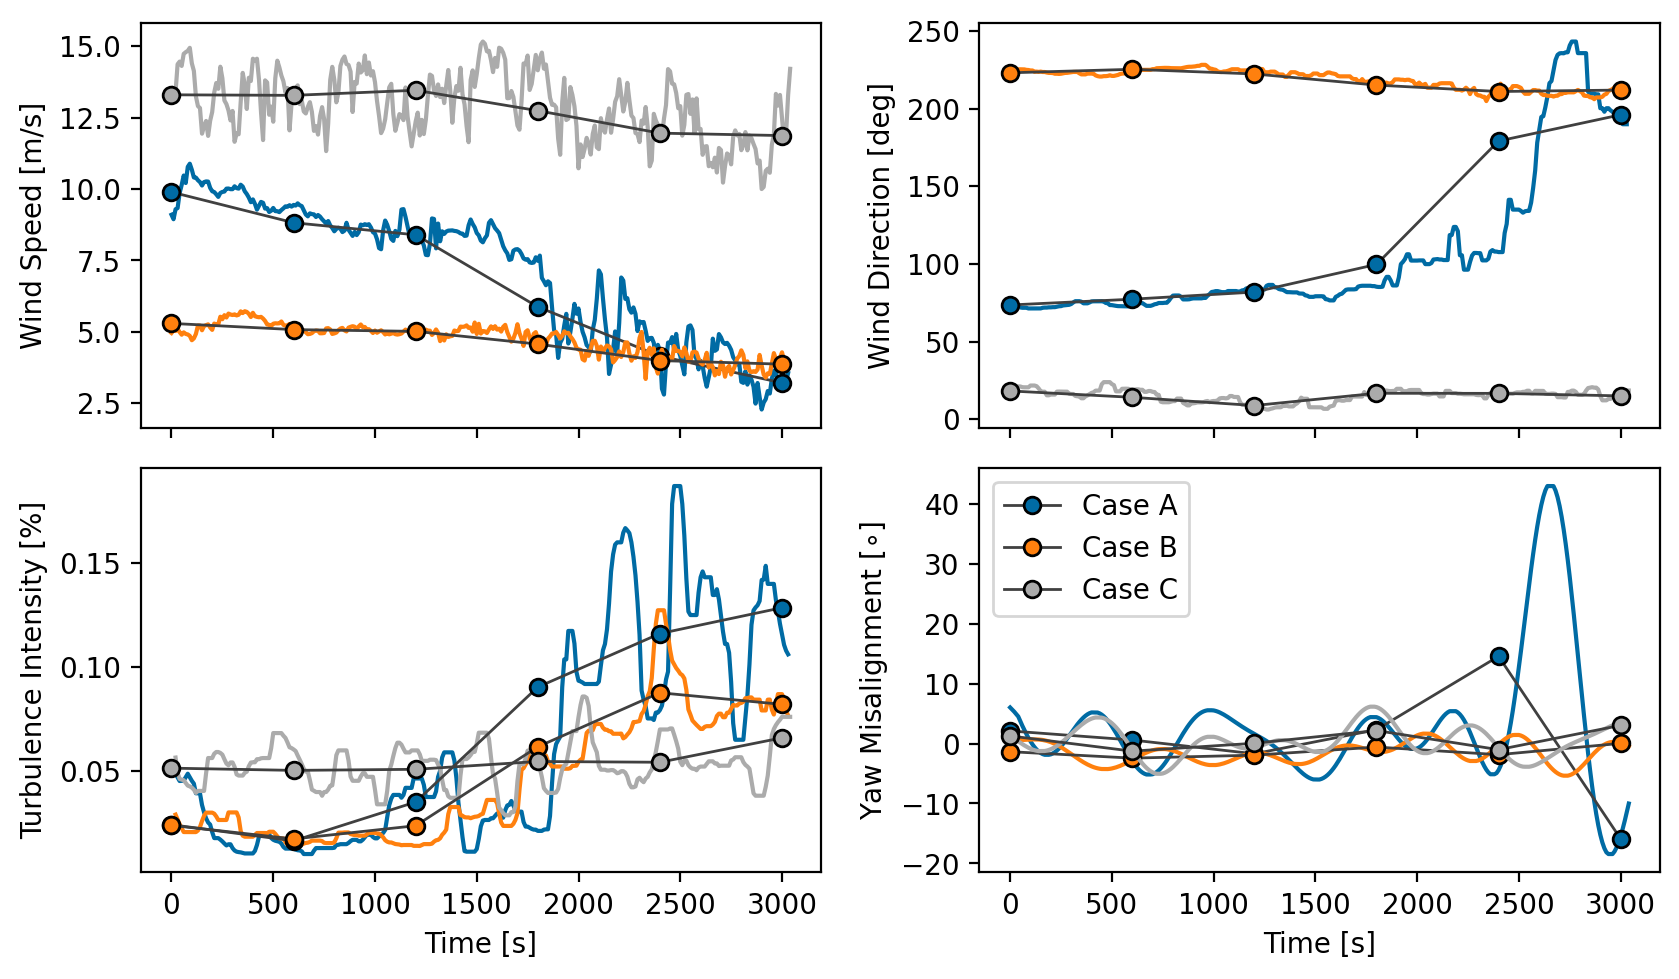
\includegraphics[width=\columnwidth]{figs/inflow_20210812.png}
    \caption{Wind speed (top left), wind direction (top right), and turbulence intensity (bottom left) recorded by the sonic anemometer at 50 m AGL. Yaw misalignment (bottom right) calculated as the difference between the nacelle heading and wind direction.}
    \label{fig:inflow}
\end{figure}

% \begin{figure}[htbp]
%   \centering
%   \begin{subfigure}[b]{0.48\columnwidth}
%     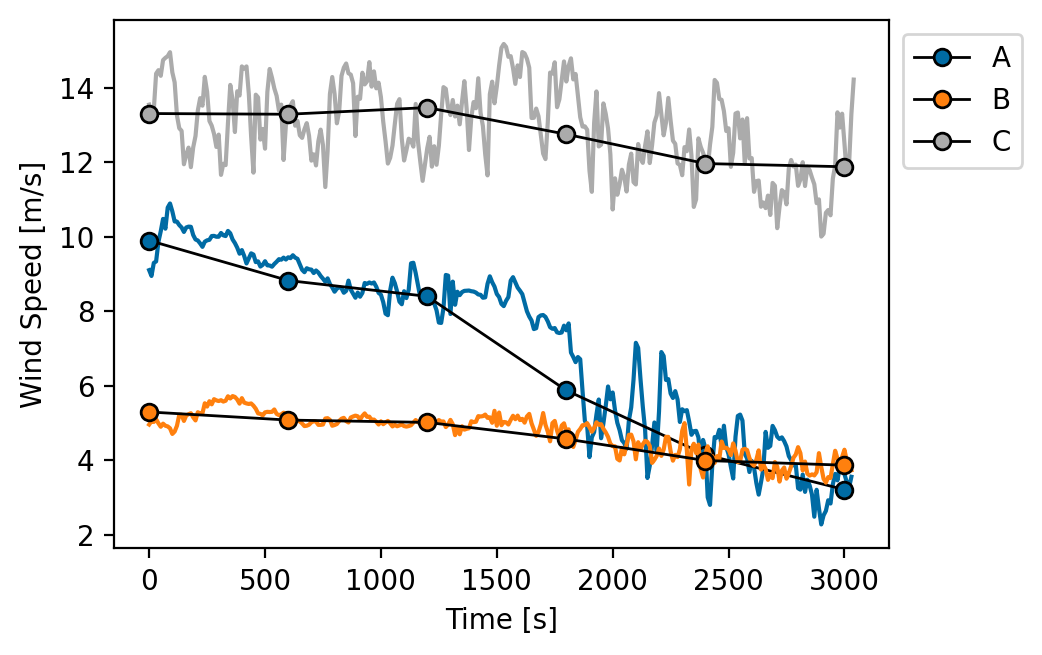
\includegraphics[width=\columnwidth]{figs/windspeed.png}
%   \end{subfigure}
%   \begin{subfigure}[b]{0.5\columnwidth}
%     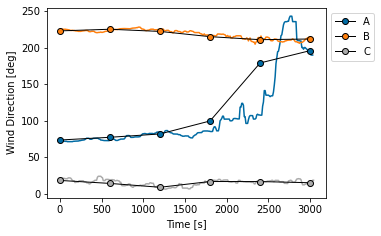
\includegraphics[width=\columnwidth]{figs/winddirection.png}
%   \end{subfigure}
%   \caption{Wind speed (left) and wind direction (right) recorded by the sonic anemometer at 50 m AGL.}
%   \label{fig:wswd}
% \end{figure}

The integral time scale for each case was calculated on a rolling 10-min basis from the horizontal wind speed reported by the sonic anemometer at 50 m AGL, including 1200 samples to estimate $T$ at each time. 
\Cref{fig:ts} shows the distribution of $T$ for each case as box and whisker plots.
In this work, the integral time scales, $T$, are taken as the characteristic period of the fluctuation in the velocity field and are used to define the characteristic frequency of turbulent fluctuations in the discussion of meandering frequencies. 
In each box plot, the whiskers extend to the maximum and minimum of each distribution and the line in the boxes denote median values of $T$ for each case.

\begin{figure}[h]
    \centering
    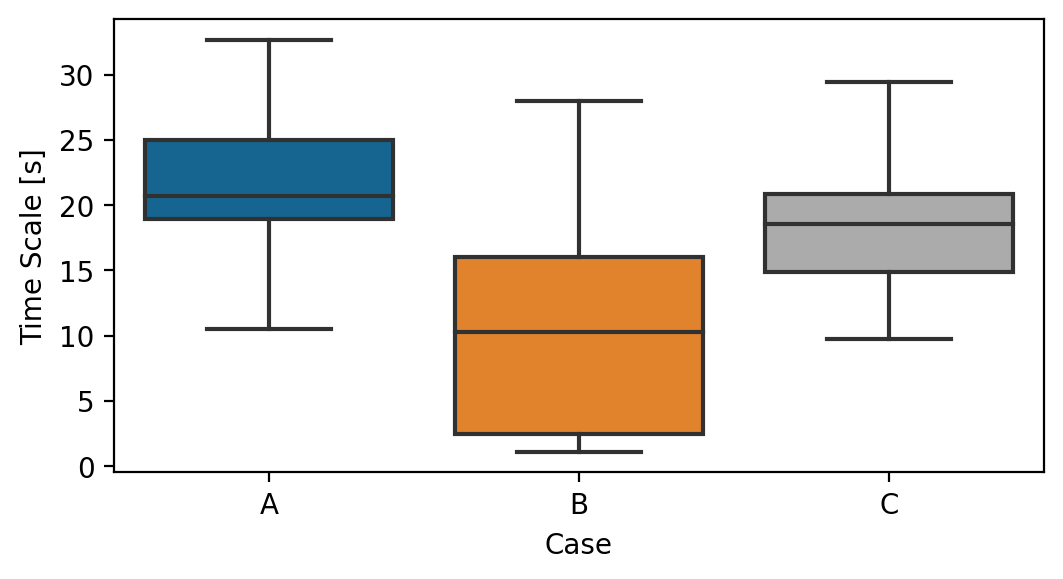
\includegraphics[width=0.5\textwidth]{figs/time_scale_box.png}
    \caption{Distributions of the integral time scale $T$ for each case. }
    \label{fig:ts}
\end{figure}

\Cref{fig:avescan} shows the time-averaged streamwise velocity field computed from the lidar scans, $\overline{u}$, for each Case Along with the detected wake center.
The average for each case contains information from 397 lidar scans. 
The detected wake centers (shown with white markers) are fit to the mean flow field and show that the wake for each case remains fairly well aligned with the mean wind direction (from right to left in the figures).
Notably, the mean field for Case A (left) shows the influence of a nearby wake in the lower left corner of the contour plot.
This second wake is not accounted for in the wake center detection method, and results in the fitted center location drifting to lower values of $y/D$ in particular scans. 
The mean flow field in Case B is well aligned with the mean flow direction throughout the entire scan region.
In Case C, the wake is slightly askew from the mean wind direction, highlighted by the detected wake centers tending toward negative values of $y/D$.


\begin{figure}[h]
  \centering
  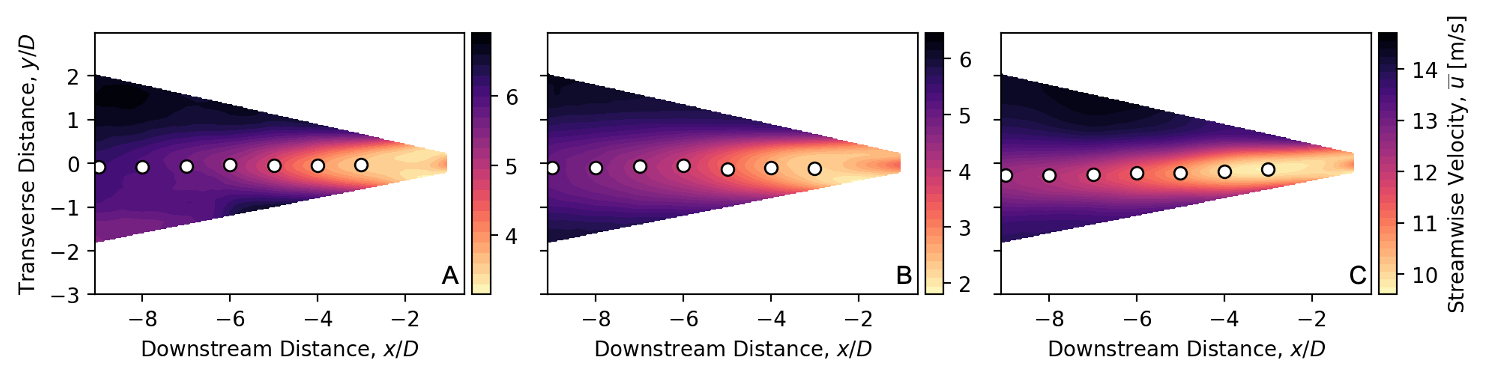
\includegraphics[width=\columnwidth]{figs/mean_scans_20210810.png}
  \caption{Time-averaged flow field from lidar scans and detected wake centers for cases A, B, and C}
  \label{fig:avescan}
\end{figure}

% section Data (end)

%%%%%%%%%%%%%%%%%%%%%%%%%%
\section{Results} % (fold)
\label{sec:Results}
%%%%%%%%%%%%%%%%%%%%%%%%%%

The mean wake centerline for each case differs depending on how it is derived: either by applying the Gaussian fit to each scan individually and then averaging collection of fit center locations across all scans (\Cref{fig:wakecenter}, crosses) or by considering wake centers in  ensembles, averaging 10-minute wake centers together to obtain a final value (\Cref{fig:wakecenter}, circles).  
In Cases A and B, the average wake center location considering 10-min ensembles is consistently more shifted toward the left looking downstream (negative values of $y/D$) than the estimate of the time-averaged location, while the opposite is true for Case C. For Cases A and C, the two methods disagree by approximately 6.7 m and 21 m, respectively, occurring at $x/D=9$ for each case.
For Case B, the maximum disagreement between the time averaged and 10-min ensemble mean estimates of wake center is 9.8 and occurs at $x/D=5$.
The differences in wake center estimates between the two methods demonstrates the unsteadiness in the flow field, which can push even the wake outside of the lidar field of view, make adjacent wakes appear in the field of view, or increase wake dissipation. 

% Differences are very small for Case C, slightly larger for Case B and largest for Case A, following the variability in the inflow for each case. 
% The change in wind direction in Case A is followed by a brief yaw misalignment as great as 40$^\circ$, while the turbine controller adjusts to new operating point. 
During the period of change in wind direction in Case A, the lidar, which is in a fixed orientation relative to the turbine nacelle, sees the wake shift toward negative values of $y/D$, especially at greater downstream distances.
Despite the change of wind direction, the average wake centers for Case A shown in \cref{fig:wakecenter} are within $y/D \le -0.15$, confirming that the wake is not biased toward either side.
Instead, the variability in atmospheric conditions for Case A are shown through the large standard deviation.
The inflow Case B shows very little change in wind direction and yaw misalignment during the record.
However, the overall and 10-min ensemble averaged wake centers show the greatest deflection in \cref{fig:wakecenter}, although the mean wake centers remain within $y/D \le -0.27$.


\begin{figure}[htb]
  \centering
  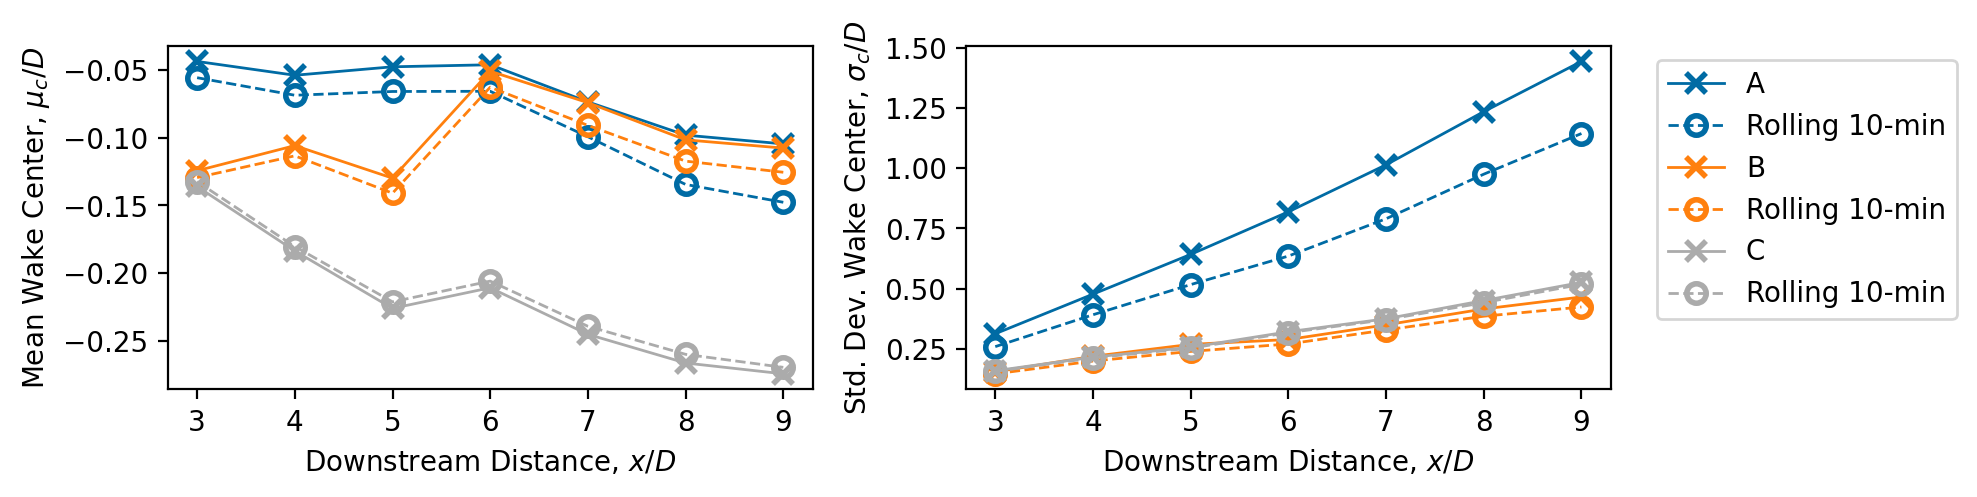
\includegraphics[width=0.95\textwidth]{figs/wake_center_mean_and_std_20210810.png}
  \caption{Mean (left) and standard deviation (right) of detected wake center locations from lidar scans.}
  \label{fig:wakecenter}
\end{figure}

The difference between the 10-minute average and wake center locations and the average of the full datasets for each case are highlighted by the time series of detected wake centers for each case in \cref{fig:wakecenterts}.
Most evident in Case A, the variability in detected weight center is not consistent throughout the time series. 
In Case A, large changes in detected wake center from scan to scan are shown for the latter half of the time series. 
% As a whole, the average center location at $x/D\in[3,6,9]$ is approximately $y=-10$ m. 
% Breaking the time series into 10-minute segments, the standard deviations of detected wake centers are considerably lower than the full time average for each case.
\begin{figure}[h]
  \centering
  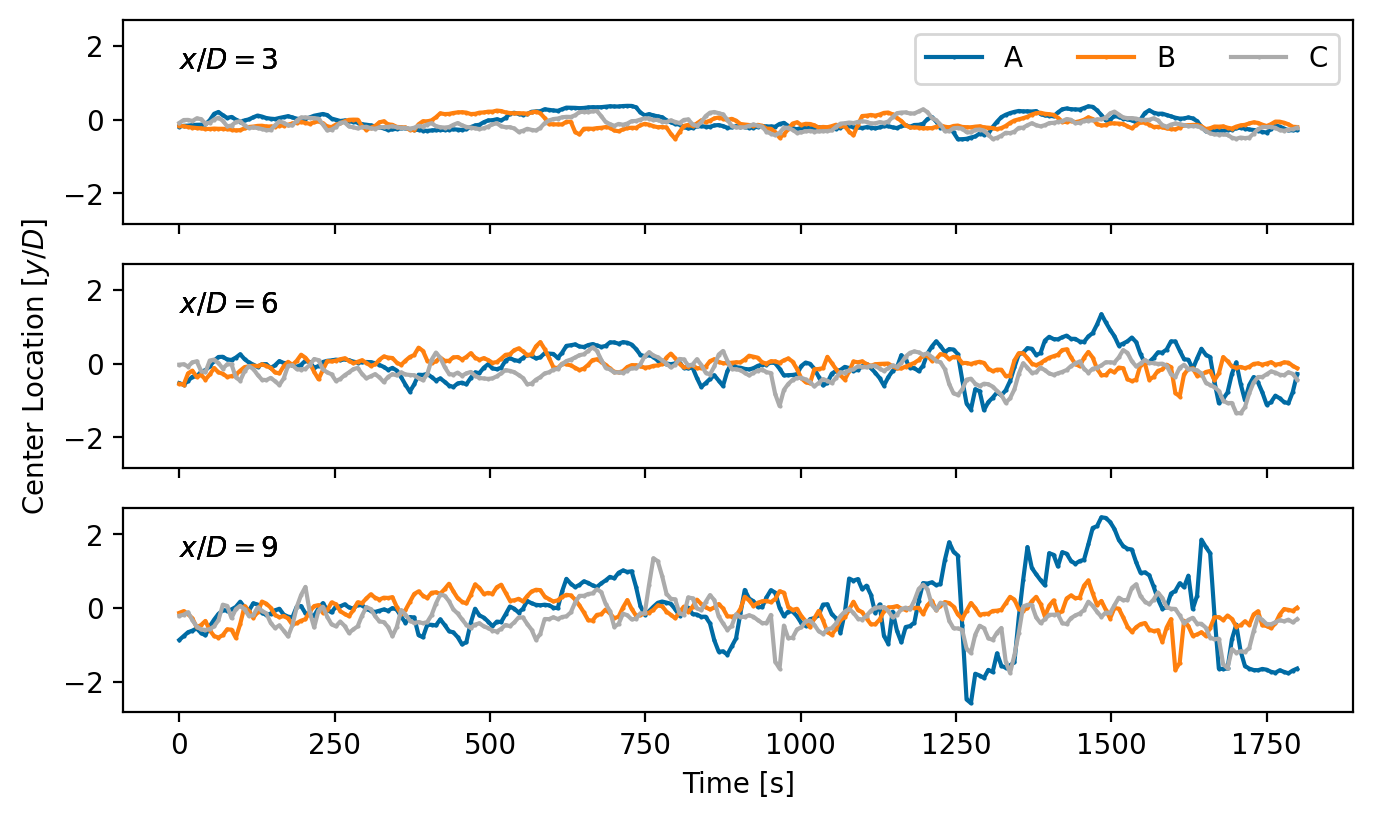
\includegraphics[width=0.95\textwidth]{figs/center_locations_xD_20210812.png}
  \caption{Time series of detected wake centers at $x/D\in[3,6,9]$ (from top).}
  \label{fig:wakecenterts}
\end{figure}

The distribution of wake center locations at each downstream position for Case C are shown in \cref{fig:centerdist}.
Moving from $x/D=3$ (yellow) to $x/D=9$ (purple), the distribution of $\mu$ flattens out, indicating that far from the wind turbine, there is more variation in wake center locations.
This is not surprising given that the wake is generated at the wind turbine, and large scale turbulent motions may interact with the wake to a greater extent farther downstream.
As the wake advects downstream, the momentum deficit region also tends to break up into smaller structures. 
This results in a fit of the wake center that is more prone to sudden jumps from one area to another, contributing to the spread shown in \cref{fig:centerdist}.
% Gaussian profile more difficult to fit in a meaningful way. 
\begin{figure}[h]
  \centering
  \begin{subfigure}[b]{0.475\columnwidth}
    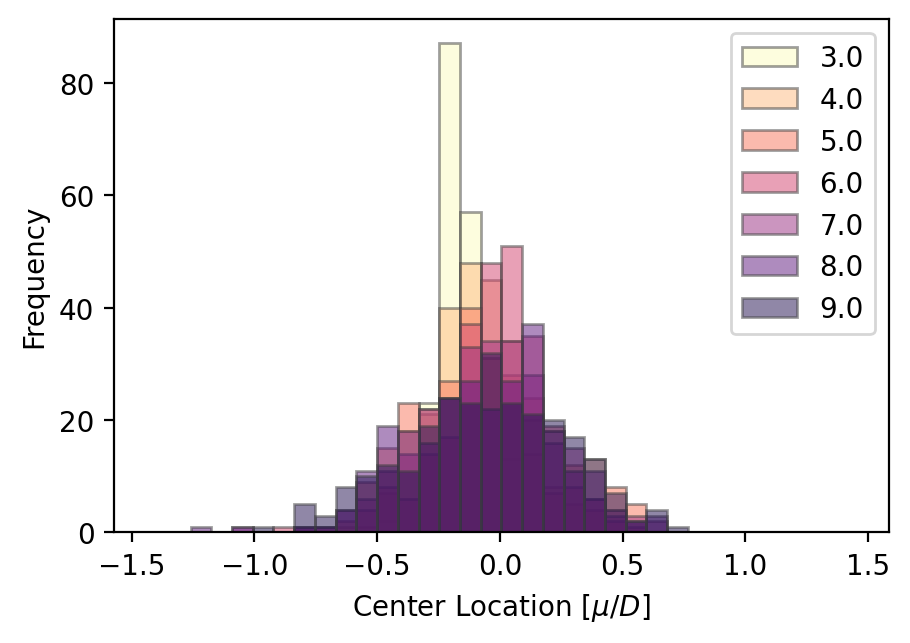
\includegraphics[width=\columnwidth]{figs/center_locations_distribution_B_20210818.png}
    \caption{Distribution of detected center locations downstream of the turbine in Case C.}
    \label{fig:centerdist}
  \end{subfigure}
  \hfill
  \begin{subfigure}[b]{0.475\columnwidth}
    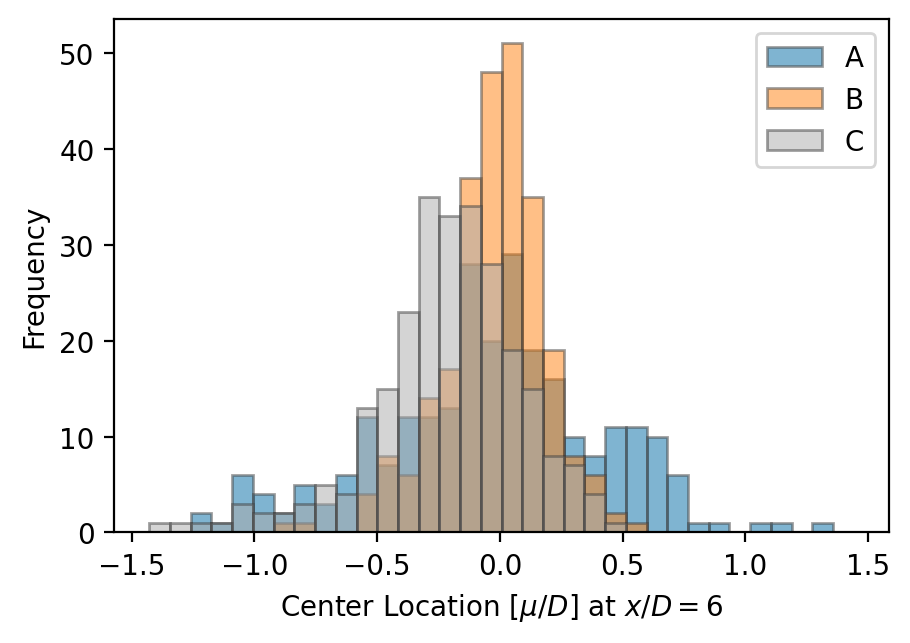
\includegraphics[width=\columnwidth]{figs/center_locations_distribution_comparison_20210818.png}
    \caption{Comparison of wake center distributions for all cases}
    \label{fig:centerdistcomp}
  \end{subfigure}
  \caption{The detected wake centers for each case vary as with downstream distance (left) and operating conditions (right).}
  \label{fig:hists}
\end{figure}
\Cref{fig:centerdistcomp} compares the distributions of wake center locations at $x/D=6$ for each case.
Echoing the time series shown in \cref{fig:wakecenterts} the distribution of Case B shows the least spread, taken here to indicate less wake meandering. 
Case C shows an intermediate level of meandering, and Case A a high level.

%Wake meandering is quantified in a single aggregate metric as the standard deviation of the detected wake center locations through each case,
% \begin{equation}
%   \sigma_c(x/D) = \sqrt{\frac{\sum_{i=1}^N \left(\mu(x/D, t) - \overline{\mu(x/D, t)}\right)^2}{N}}
%   \label{eq:meandermetric}
% \end{equation}

%%%%%%% Should this be a new subsection?
When reconstructing the velocity field with POD modes, we seek to match as closely as possible the standard deviation of wake center locations from the reconstructed flow field ($\hat{\sigma}_c$) to that of the original flow field ($\sigma_c$).
Combinations of modes that accurately reproduce wake meandering for each case (i.e. $\sigma_c\approx\hat{\sigma}_c$) are taken to represent wake meandering in the low-order representation of the velocity field. 

Each case requires a different number of modes to represent a given threshold of the TKE in the basis of lidar scans
%(\Cref{fig:eig,fig:cumsum}), 
arising from the fact that each case reflects different impacts of large-scale turbulence. 
Noted in Table \ref{tab:modes}, Case A requires only a single mode to represent more than 50\% of the input TKE (the zeroth mode, $\phi^{(0)}$, is the time-averaged flow field) and requires only 24 modes to reach 95\% of the TKE.
In contrast, Case B requires many more modes to reach the same thresholds of TKE. 
This trend corresponds to the distributions shown in \cref{fig:centerdistcomp}: greater values of $\sigma_c$ indicate that fewer POD modes are required to represent a given threshold of TKE, as seen for Case A.
\Cref{fig:PODeig} shows the distribution of energy described by the POD eigenvalues for each case. 

\begin{table}[htb]
  \centering
  \caption{Number of modes required to reach the listed threshold [\%] of TKE for each case.}
  \label{tab:modes}
  \begin{tabular}{l|ccc}
    Case    & A & B & C \\
    \hline
    50.0 \% & 1          & 2          & 2          \\
    75.0 \% & 3          & 16         & 8          \\
    90.0 \% & 10         & 57         & 29         \\
    95.0 \% & 24         & 103        & 56         \\
    % 99.0 \% &  88 &  229 &  150 \\         
  \end{tabular}
\end{table}

\begin{figure}[h]
    \centering
    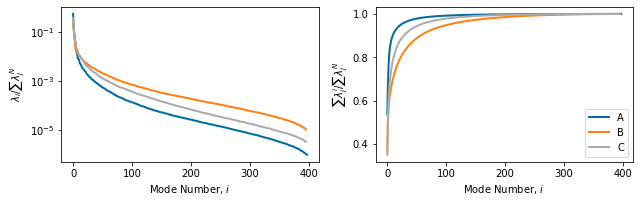
\includegraphics[width=\columnwidth]{figs/eigenvalues_20210818.png}
    \caption{Distribution of TKE described by the normalized eigenvalues of the POD (left) and their cumulative summation (right).}
    \label{fig:PODeig}
\end{figure}
% \begin{figure}[h]
%   \centering
%   \begin{subfigure}[b]{0.475\columnwidth}
%     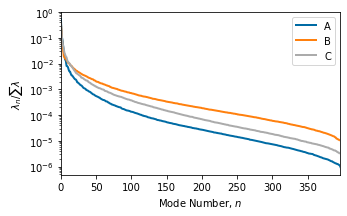
\includegraphics[width=\columnwidth]{figs/eigenvalues_constantmean.png}
%     \caption{Normalized POD eigenvalues}
%     \label{fig:eig}
%   \end{subfigure}
%   \hfill
%   \begin{subfigure}[b]{0.475\columnwidth}
%     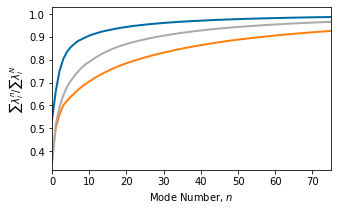
\includegraphics[width=\columnwidth]{figs/eigenvalues_sumsum_constantmean.png}
%     \caption{Cumulative summation of eigenvalues}
%     \label{fig:cumsum}
%   \end{subfigure}
%   \caption{Distribution of TKE described by the eigenvalues of the POD.}
%   \label{fig:PODeig}
% \end{figure}

The full span of modal basis described by the POD does not converge evenly. Lower-rank modes describe turbulent structures represented in more observations, by definition, and converge faster. Higher ranking modes represent less coherent structures, and require a larger sample size to be statistically converged. \Cref{fig:convergence} contains the results of a convergence test that compares the variability of POD modes constructed from randomly sampled snapshots within the set of observations, averaging over all three test cases. The mode error, $\varepsilon_{\phi^{(i)}}$, shown in \cref{fig:convergence} is defined as the standard deviation of POD modes defined with a randomly selected sample of $N$ snapshots. For each basis size $N$, up to 1000 subsets of observations were used to define POD bases, offering a statistical view of the structures described by the POD modes. 

\begin{figure}[htb]
    \centering
    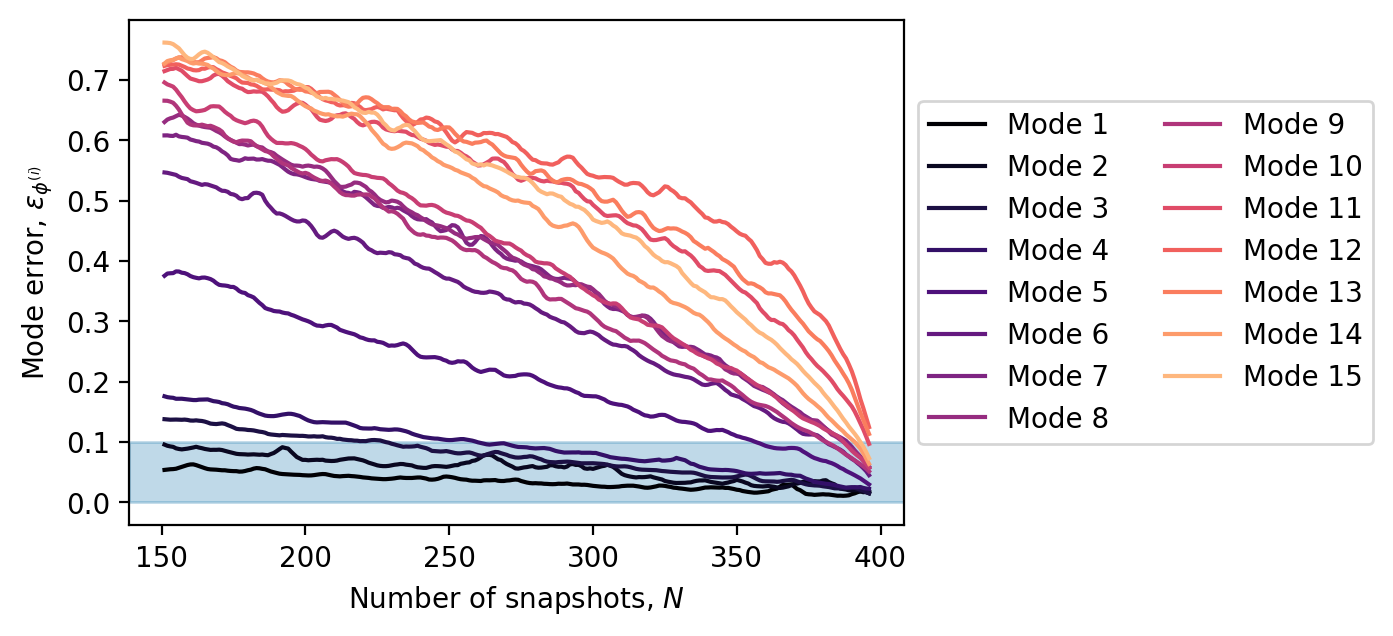
\includegraphics[width=0.85\textwidth]{figs/convergence_std.png}
    \caption{Convergence of POD modes with increasing observational sample size. Blue region represents region where the mode error is less than 10\% and is considered converged.}
    \label{fig:convergence}
\end{figure}

Only the first 15 modes, containing the most coherent structures observed in the lidar scans, are considered in the flow field reconstruction for meandering analysis. \Cref{fig:convergence} shows that there is little variability in the first 4 POD modes for sets of $\sim275$ observations or more, at which point the mode error $\varepsilon_{\phi^{(i)}}$ stays below 10\% highlighted as a blue region in the figure.
Here, we choose 10\% as the error threshold that identifies when statistical convergence is reached for each mode number.
Each case contains 396 modes (defined with 396 snapshots), ensuring that most of the modes considered in the meandering study reach acceptable statistical convergence.
The only exceptions to the convergence requirement are modes 12 and 13, which reach a convergence level of $\varepsilon_{\phi^{(12)}}=12.5\%$ and $\varepsilon_{\phi^{(13)}}=11.3\%$.
Although these two modes do not fall below the 10\% threshold, \cref{fig:convergence} indicates that both are converging quickly, and are unlikely to misrepresent the wake turbulence in any way that is detrimental to the study.

In reconstructing the flow field as in \cref{eq:PODset}, the sets of modes used to describe the turbulence included between 3 and 15 POD modes, plus the zeroth mode representing the mean flow.
For each set size, all possible mode combinations were tested (see Table \ref{tab:comb}), producing a large sample of reconstructed wakes.
For each combination, the wake profiles were fit to the Gaussian function in \cref{eq:gaussfit}, and the standard deviation of the reconstructed flow field, $\hat{\sigma}_c$, was estimated, leading to thousands of low-order estimates of the wake center at each downstream position for each case.

\Cref{fig:delta_std} shows the distribution of the difference between the original wake center standard deviation and that of the the lower order reconstruction,
\begin{equation}
  \Delta \sigma_c = \sigma_c - \hat{\sigma}_c
  \label{eq:delta)std}
\end{equation}
Each box and whisker plot in \cref{fig:delta_std} represents the range of $\Delta \sigma_c$ for a particular maximum number of modes $k$ throughout the wake. 
Values of $\Delta \sigma_c$ close to zero indicate that a particular combination of modes accurately represents the wake meandering statistics.
For all values of $k$, $\Delta \sigma_c$ increases with $x/D$, indicating that the variability in wake center location downstream of the turbine is more difficult to accurately represent than near the turbine.
It is also clear from the figure that using a larger number of modes shifts the bulk of the distributions of $\Delta \sigma_c$ toward zero, improving the representation of wake meander.
Notably, when $k=8$ or $k=12$, there are more outlier values of $\Delta \sigma_c$ in the far wake of Cases A and C and more cases that overshoot the target of $\Delta \sigma_c=0$, indicating that there are particular combinations of POD modes that over represent the wake meander in those cases.

\begin{figure}[h]
    \centering
    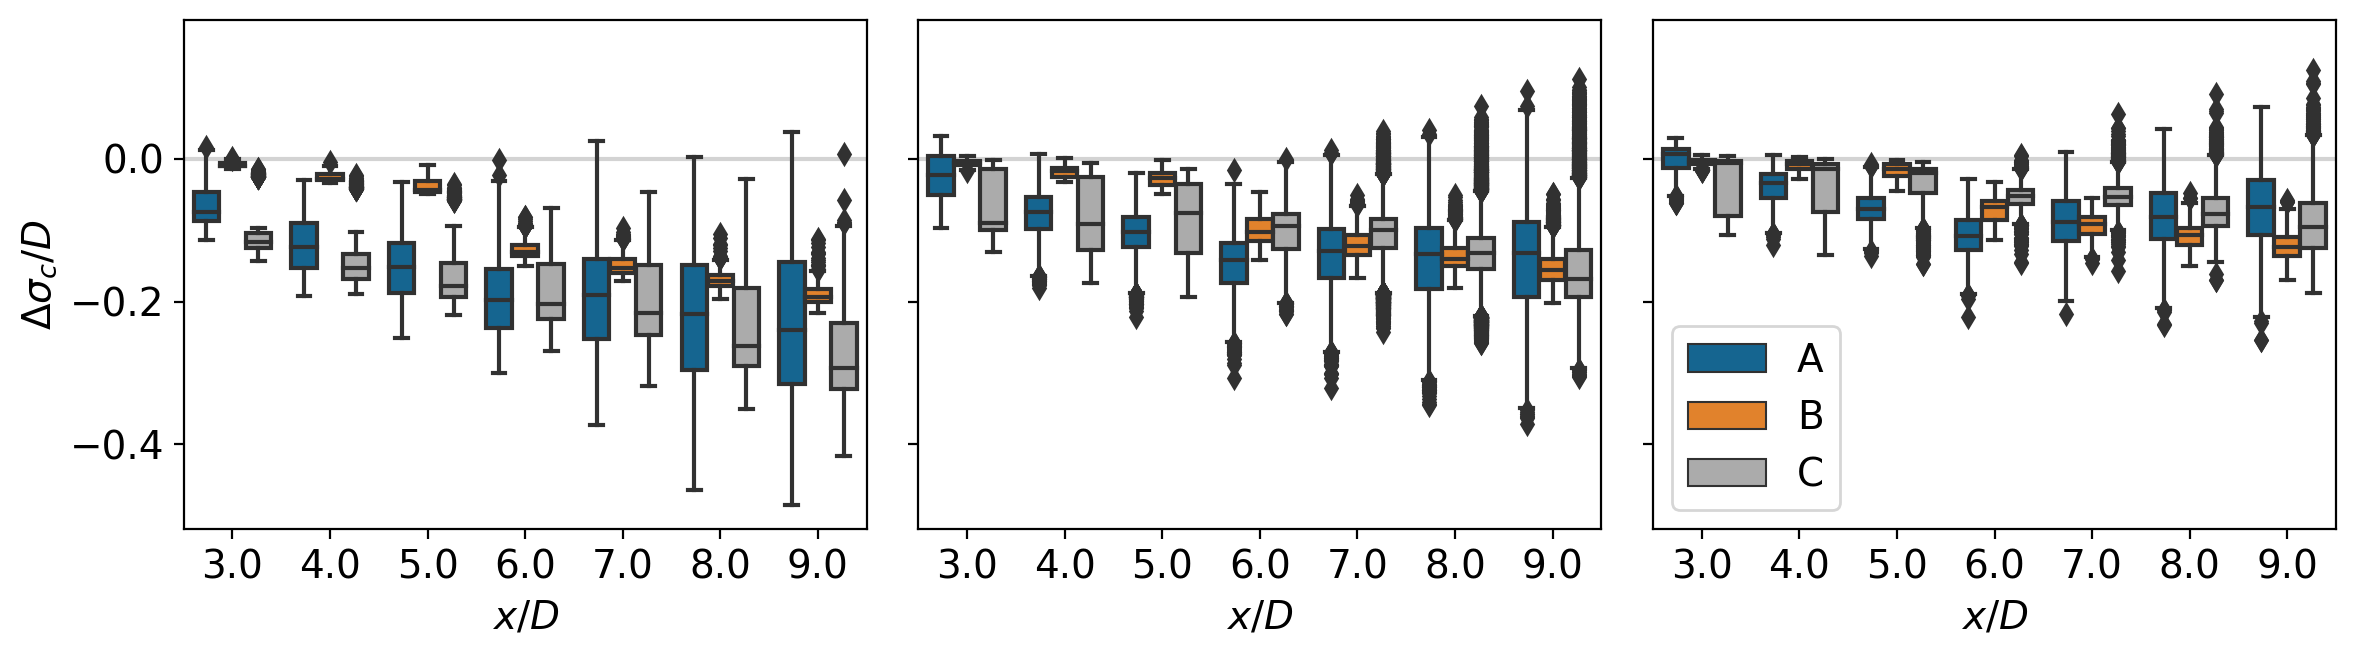
\includegraphics[width=\columnwidth]{figs/delta_std_boxplots_20210818.png}
    \caption{Distribution of the change in wake center standard deviation for up to $k\in[4,8,12]$ modes (from left).}
    \label{fig:delta_std}
\end{figure}
% \begin{figure}[h]
%   \centering
%   \begin{subfigure}[b]{0.49\columnwidth}
%     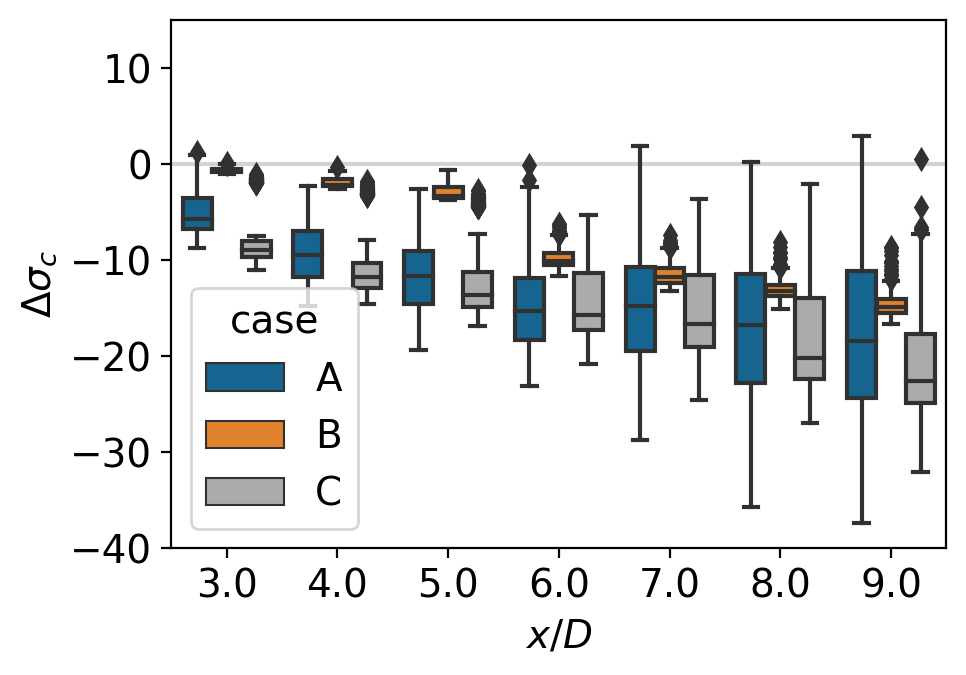
\includegraphics[width=\columnwidth]{figs/delta_std_boxplots_xd4.png}
%     \caption{$k=4$}
%     \label{fig:energy_ratio}
%   \end{subfigure}
%   \begin{subfigure}[b]{0.49\columnwidth}
%     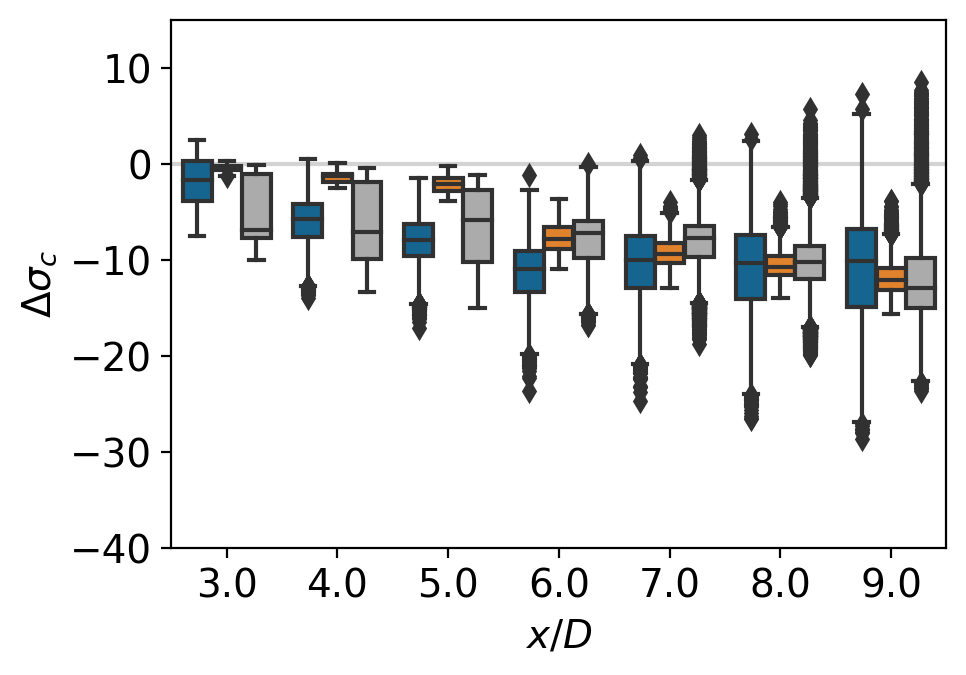
\includegraphics[width=\columnwidth]{figs/delta_std_boxplots_xd8.png}
%     \caption{$k=8$}
%     \label{fig:energy_ratio_lowtvar}
%   \end{subfigure}
%   \begin{subfigure}[b]{0.49\columnwidth}
%     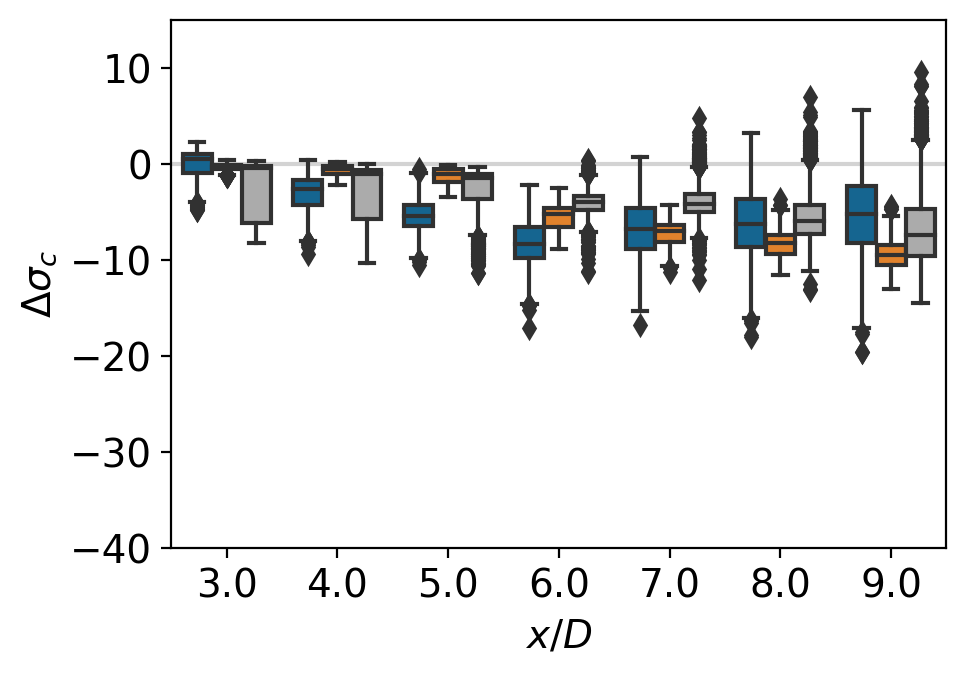
\includegraphics[width=\columnwidth]{figs/delta_std_boxplots_xd12.png}
%     \caption{$k=12$}
%     \label{fig:T3_energy_ratio_comp}
%   \end{subfigure}
%   \caption{Distribution of the change in wake center standard deviation for up to $N\in[4,8,12]$ modes.}
%   \label{fig:delta_std}
% \end{figure}

In a general sense, wake meandering in Case B appears to be more accurately reproduced through POD reconstruction.
However, beyond $x/D = 5$, there are  particular combinations of modes that very accurately represent Cases A and C, even while the majority of combinations do not.
Table \ref{tab:minerr} shows the best outcome for each case at each downstream position in terms of $\Delta \sigma_c$. 
For $x/D \le 5$, Case B exhibits the lowest values of $\Delta \sigma_c$; for $x/D \ge 6$, Case B exhibits higher values of $\Delta \sigma_c$ than the best mode combinations for either Case A or C.  

\begin{table}[htb]
  \caption{Change in the standard deviation of detected wake center and the number of modes required for the best-fit field reconstructions}
  \label{tab:minerr}
  \centering
  \begin{tabular}{c|cccccc}
    Case  & \multicolumn{2}{c}{A} & \multicolumn{2}{c}{B} & \multicolumn{2}{c}{C}                                        \\
    \hline
    $x/D$ & $\Delta\sigma_c/D$     & N Modes               & $\Delta\sigma_c/D$      & N Modes & $\Delta\sigma_c/D$ & N Modes \\
    % \midrule
    \hline
 3.0 &          -0.000005 &     3.0 &       9.234049e-08 &     9.0 &          -0.000003 &     7.0 \\
4.0 &           0.000067 &     5.0 &      -2.449069e-06 &     9.0 &          -0.000136 &     8.0 \\
5.0 &          -0.001648 &     8.0 &      -1.463068e-03 &     9.0 &          -0.003182 &     8.0 \\
6.0 &          -0.001123 &     9.0 &      -2.239742e-02 &    10.0 &           0.000250 &     9.0 \\
7.0 &           0.000064 &     9.0 &      -4.840386e-02 &    10.0 &          -0.000002 &    11.0 \\
8.0 &          -0.000009 &    10.0 &      -3.868024e-02 &    11.0 &          -0.000019 &    11.0 \\
9.0 &           0.000067 &    11.0 &      -4.507103e-02 &    12.0 &           0.000007 &    12.0 \\
  \end{tabular}
\end{table}


% \begin{figure}[h]
%     \centering
%     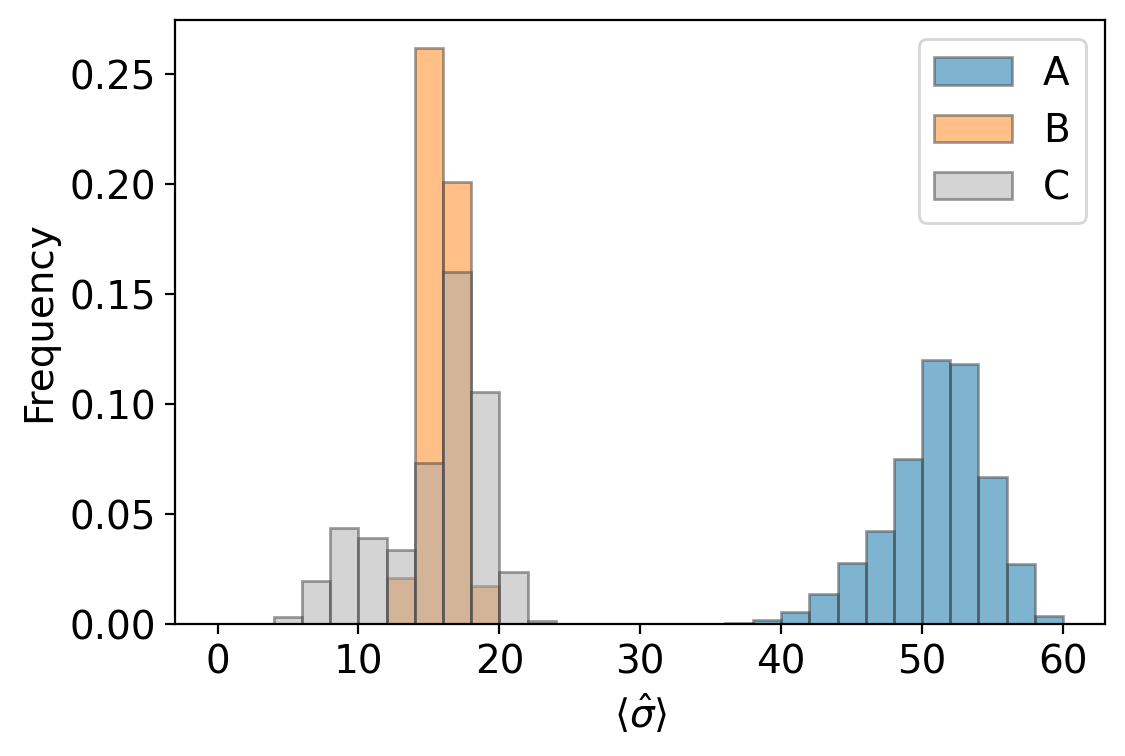
\includegraphics[width=0.45\textwidth]{figs/stdDevRec_byCase.png}
%     \caption{Each case has a distinct distribution of reconstructed wake center locations}
%     \label{fig:stdDevRec}
% \end{figure}

Table \ref{tab:minerr} points to an important observation for the current study. 
It is not always the case that adding more modes to the lower-order representation of the flow field leads to a smaller difference in the standard deviation of wake center location. 
In some cases, the meandering of the wake is more accurately described with a particular combination of fewer modes even if they represent less of the total TKE.
\Cref{fig:minDelta} highlights this observation for each of the three test cases. 
Most evident in Case A (left), in most of the wake, the best 12-mode representation of the flow is not the best predictor of wake meandering, indicating that there are higher-order modes that detract from the physics of interest.
In Case B (center) this is evident for $x/D \ge 7$ where the best 10-mode reconstruction outperforms the best 12-mode reconstruction.
For Case C (right) the representation of wake meandering with 6 to 12 modes converges at $x/D=6$. 
This is taken to indicate that the meander cannot be accurately represented with any combination of 5 modes or fewer, and that some interaction between turbulent structures leads to meandering in this case.

\begin{figure}[h]
  \centering
  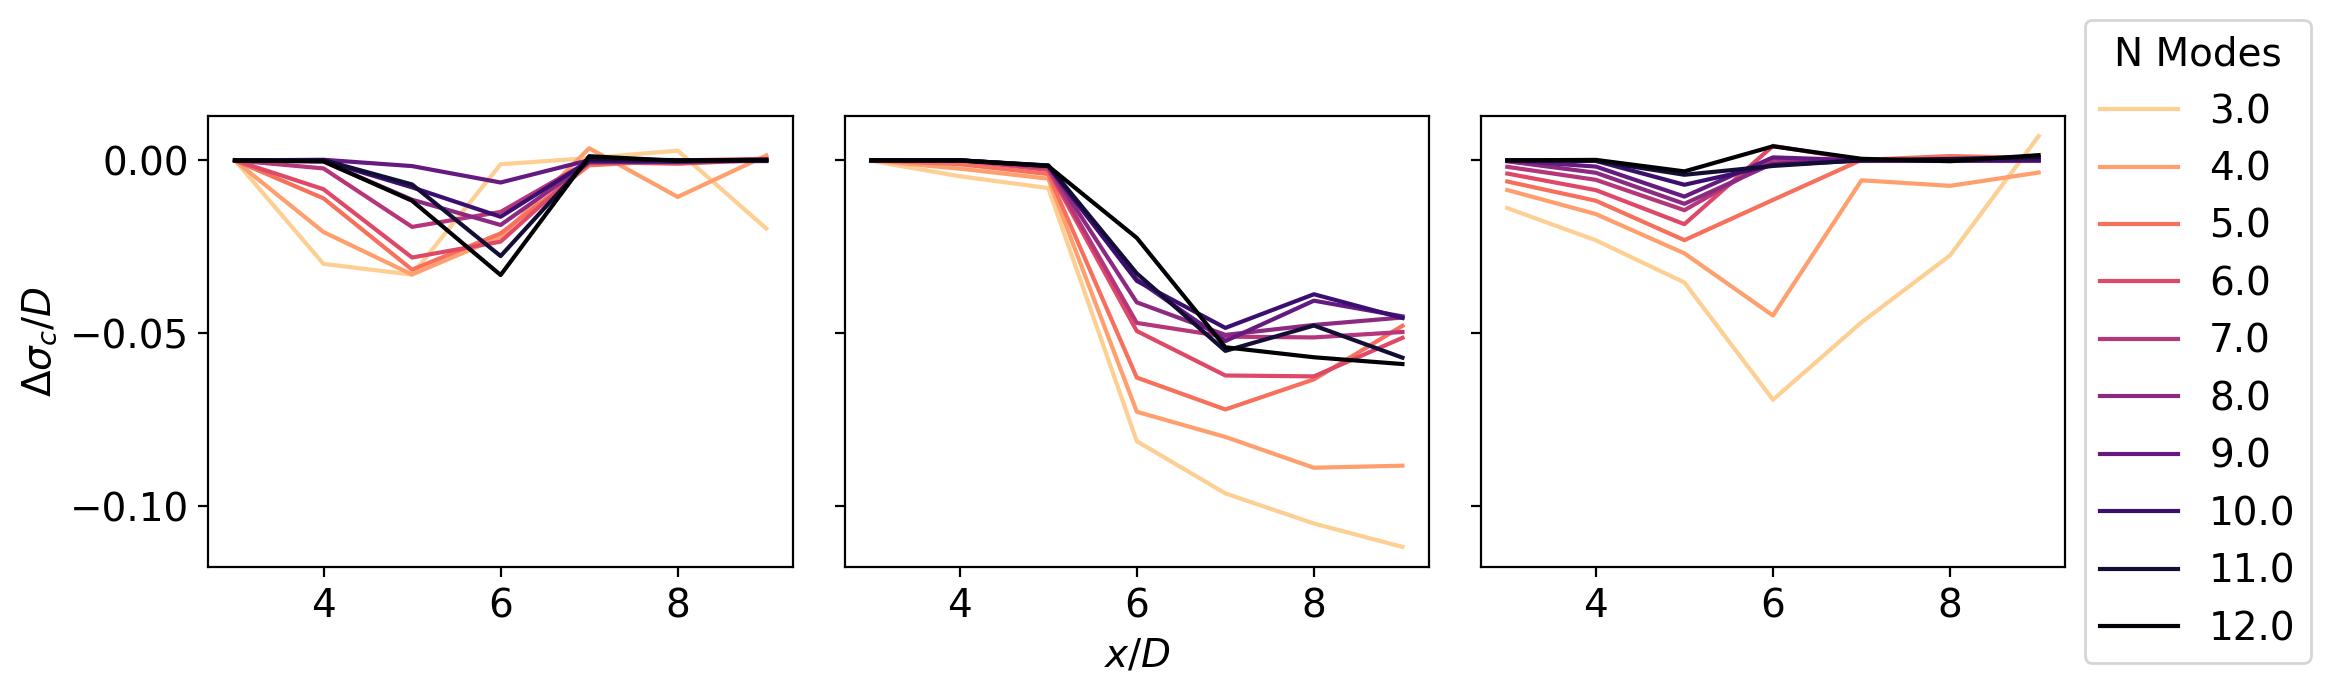
\includegraphics[width=0.95\textwidth]{figs/min_delta_stdDev_by_N.png}
  \caption{Best-fit reconstruction of wake meander for Cases A, B, and C (from left) at each downstream location varying maximum number of modes.}
  \label{fig:minDelta}
\end{figure}

Universally across the cases tested here, not every mode contributes to the accurate representation of wake meandering.
\Cref{fig:modeOccurenceInBestCases} tabulates the frequency of representation of particular POD modes in the best fit combinations for each value of $k$.
Lowest order modes, representing the largest turbulent structures, are most uniformly represented in each of the best fit combinations, with the exception of mode 2 for Case C, which is only present for half of the total combinations.
Modes 4 and 5 do not appear in any of the best fit combinations for Case B, although mode 7 is present in 9 out of 10 of the best fit combinations.
Conversely, mode 7 is not present in any of the best fit combinations for Case A.
While the modes from one case are not expected to be identical to those from any other case---given that they characterize the turbulence in different atmospheric conditions---they should represent structures of approximately the same scale. 
Inconsistent dependence on mode structures from case to case may indicate that wake meandering has a more complicated relationship with turbulence in the wake than noted in the literature. %Paula?

\begin{figure}[h]
  \centering
  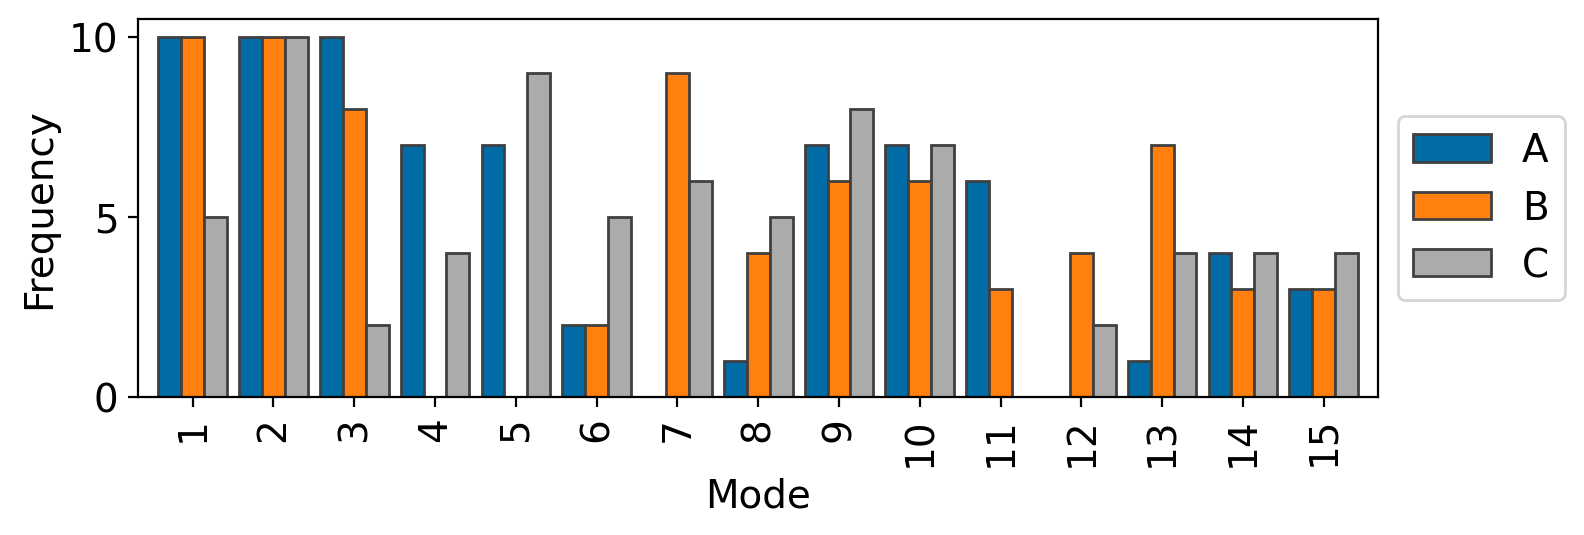
\includegraphics[width=0.75\textwidth]{figs/modeOccurenceInBestCases.png}
  \caption{Frequency of mode representation in best-fit reconstructions varying maximum number of modes.}
  \label{fig:modeOccurenceInBestCases}
\end{figure}

To assess the dependence of wake meandering statistics on particular POD modes, a linear regression test was conducted with the full suite of 30706 mode combinations for each case.
Each low-dimensional representation of the flow field is a linear combination of the product of POD modes and their respective coefficients, suggesting that the reconstructed flow field $\hat{u}$ can only be linearly dependent on each mode. 
The sensitivity of wake center location to the presence or absence of modes is highlighted through linear regression of modes (as dummy variables) to relative error of wake center standard deviation, $\varepsilon = \langle\Delta \sigma_c \rangle/ \langle\sigma_c \rangle$.
Posing the linear system,
\begin{equation}
  \bm{\varepsilon} = \bm{X}\bm{\beta} + \xi
  \label{eq:linearreg}
\end{equation}
the relative error from each combination is stacked in to the vector $\bm{\varepsilon} = [\varepsilon_1, ..., \varepsilon_K]$, the matrix $\bm{X} = [I_1, ..., I_K]$ contains the subset of modes used in each combination up to $K=30706$ for each case. 
The matrix $\bm{\beta} = [\beta_1, ..., \beta_K]$ contains the coefficients associated with each mode and the regression error is expressed as $\xi$.  
The linear regression coefficients for the modes 1 through 15 are shown in \cref{fig:regression}.
Large negative values of $\beta$ contribute most to accurately reproducing wake meander in $\hat{u}$ (i.e., they reduce error $\varepsilon$ the most) and positive values actually \emph{add} to the error associated with reconstructed wake meandering.
\Cref{fig:regression} makes it clear that in Cases B and C there are a few nonsequential structures that consistently contribute to the standard deviation of detected wake center. 
In Case B, modes 1 and 2 are the dominant contributors, followed by modes 5--11 to a lesser degree.
For Case C, modes 1, 2, and 5 are most highly correlated with wake meandering.

\begin{figure}[h]
  \centering
  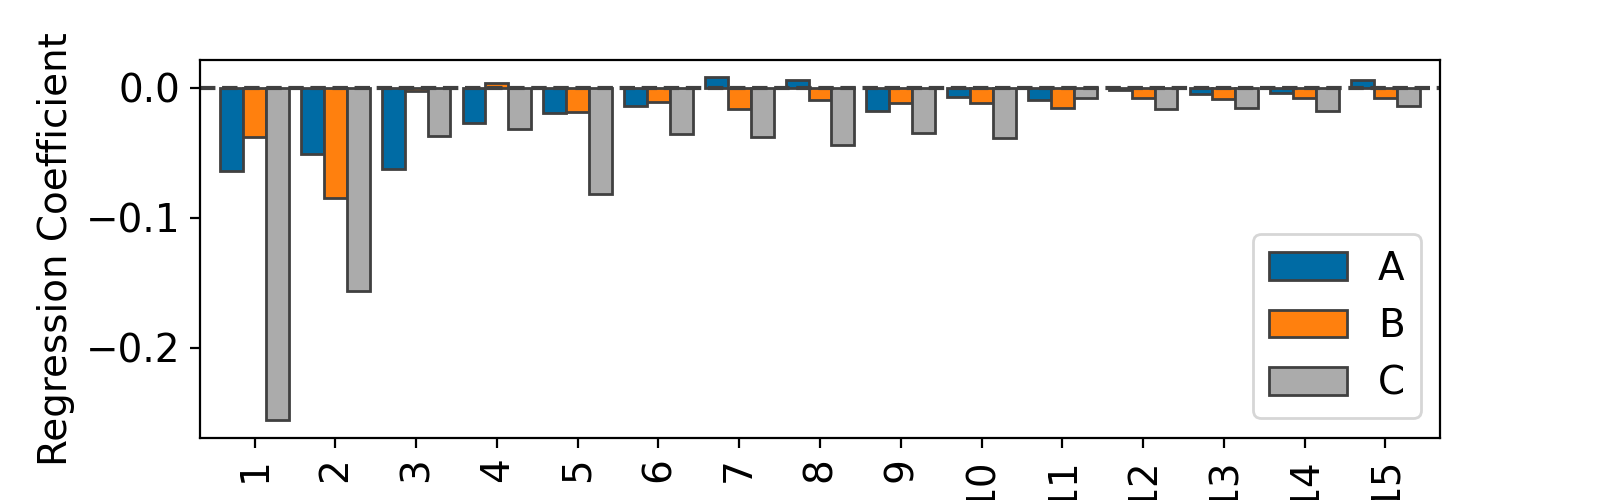
\includegraphics[width=0.78
    \textwidth]{figs/regr_coefficient.png}
  \caption{Linear regression coefficient for each mode contributing to the variability of the reconstructed wake center.}
  \label{fig:regression}
\end{figure}

\Cref{fig:bestworst} illustrates selected turbulence structures underlying the regression test results for Case C in \cref{fig:regression}. 
In the left column, modes 1, 2, and 5 are those that contribute most to the accurate reconstruction of wake meander. 
Each of the structures for modes 1, 2, and 5 occupy the full scan area and exhibit some asymmetry over the streamwise axis that contributes to the variability in the wake center location.
In the right column, the structures have a more complicated spatial character, highlighting many smaller regions within the scan area. 
When integrated into a reconstructed flow field as in \cref{eqn:nuts}, these structures do not contribute significantly to the meandering of the wake center. 

\begin{figure}[h]
  \centering
  \begin{subfigure}[b]{0.45\columnwidth}
    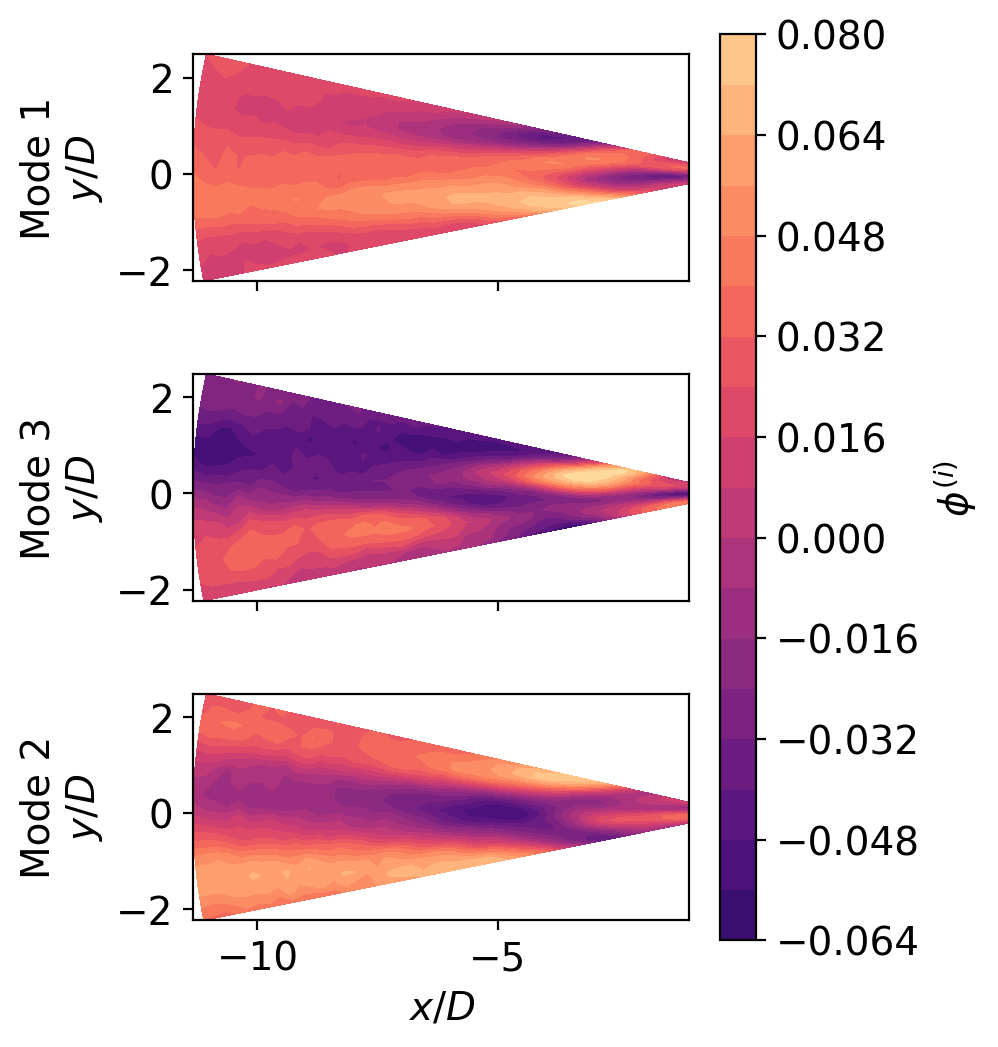
\includegraphics[width=\columnwidth]{figs/C_best_modes.png}
    % \caption{Normalized POD eigenvalues}
    % \label{fig:eig}
  \end{subfigure}
  \hspace{0.5cm}
  \begin{subfigure}[b]{0.45\columnwidth}
    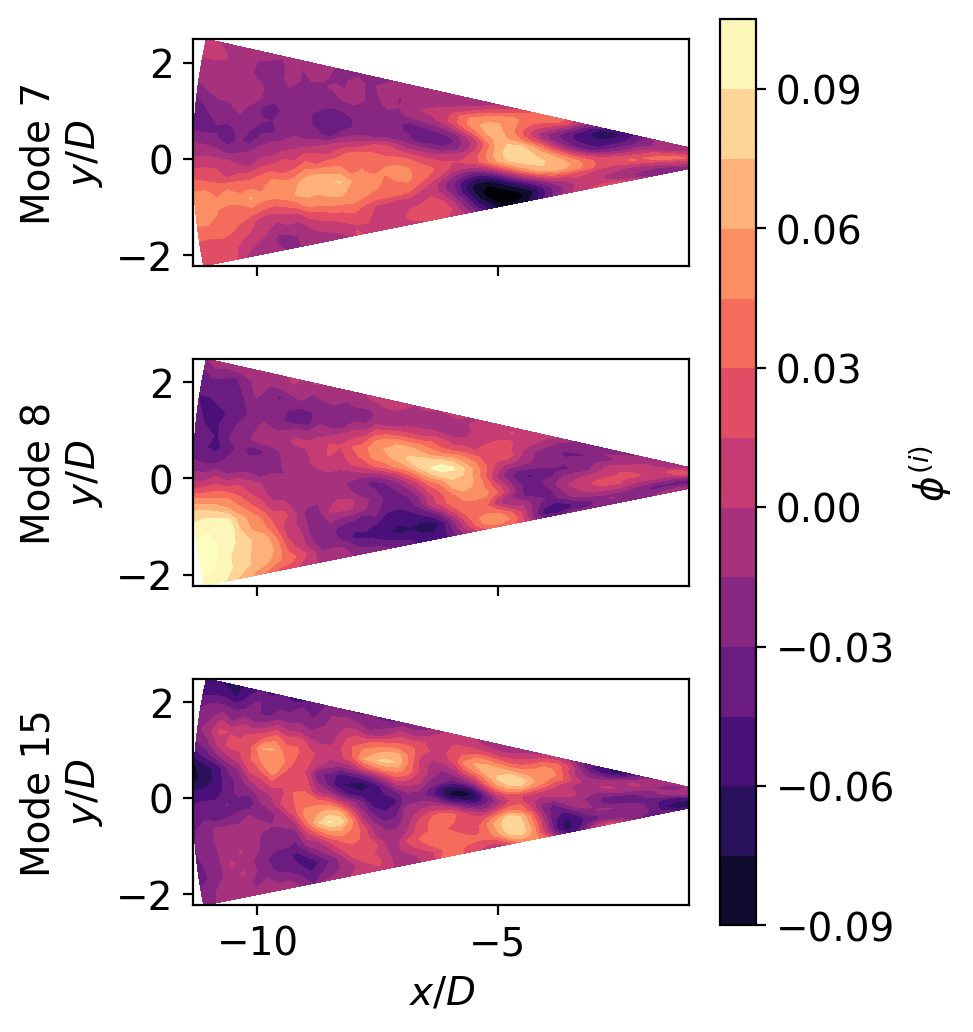
\includegraphics[width=\columnwidth]{figs/C_worst_modes_20210818.png}
    % \caption{Cumulative summation of eigenvalues}
    % \label{fig:cumsum}
  \end{subfigure}
  \caption{Modes contributing the most (left) and the least (right) to the accurate reproduction of wake meander.}
  \label{fig:bestworst}
\end{figure}



For visual verification of the regression findings presented above, \cref{fig:fieldrec} compares the velocity field from Case C presented by the lidar scan (left) to the best (center) and worst (right) reconstructions with 6 modes and the time averaged flow field.
This particular case and value of $k$ (Case C and $k=7$) was selected to highlight the differences between the best and worst combinations of modes, with the maximum difference between streamwise averaged $\Delta \sigma_c$.
In \cref{fig:fieldrec}, the contour plot denotes the velocity field, with the wake highlighted with brighter colors and freestream velocity in black.
Superimposed on the flow field, the detected wake center for this particular scan are shown with white markers.
Detected wake centers for the best reconstruction (center) closely match those of the original lidar scan, with the exception of $x/D=3$, very close to the turbine.
This in itself is interesting as the near wake was shown in \cref{fig:centerdist} to exhibit the least variability. 
That the best-fit reconstruction misses the near wake may indicate that particular modes are better suited to represent the wake center distribution near the turbine, and others better for the far wake.
The worst-fit reconstruction (right) does not accurately represent either the flow field or the wake centers. 

\begin{figure}[h]
  \centering
  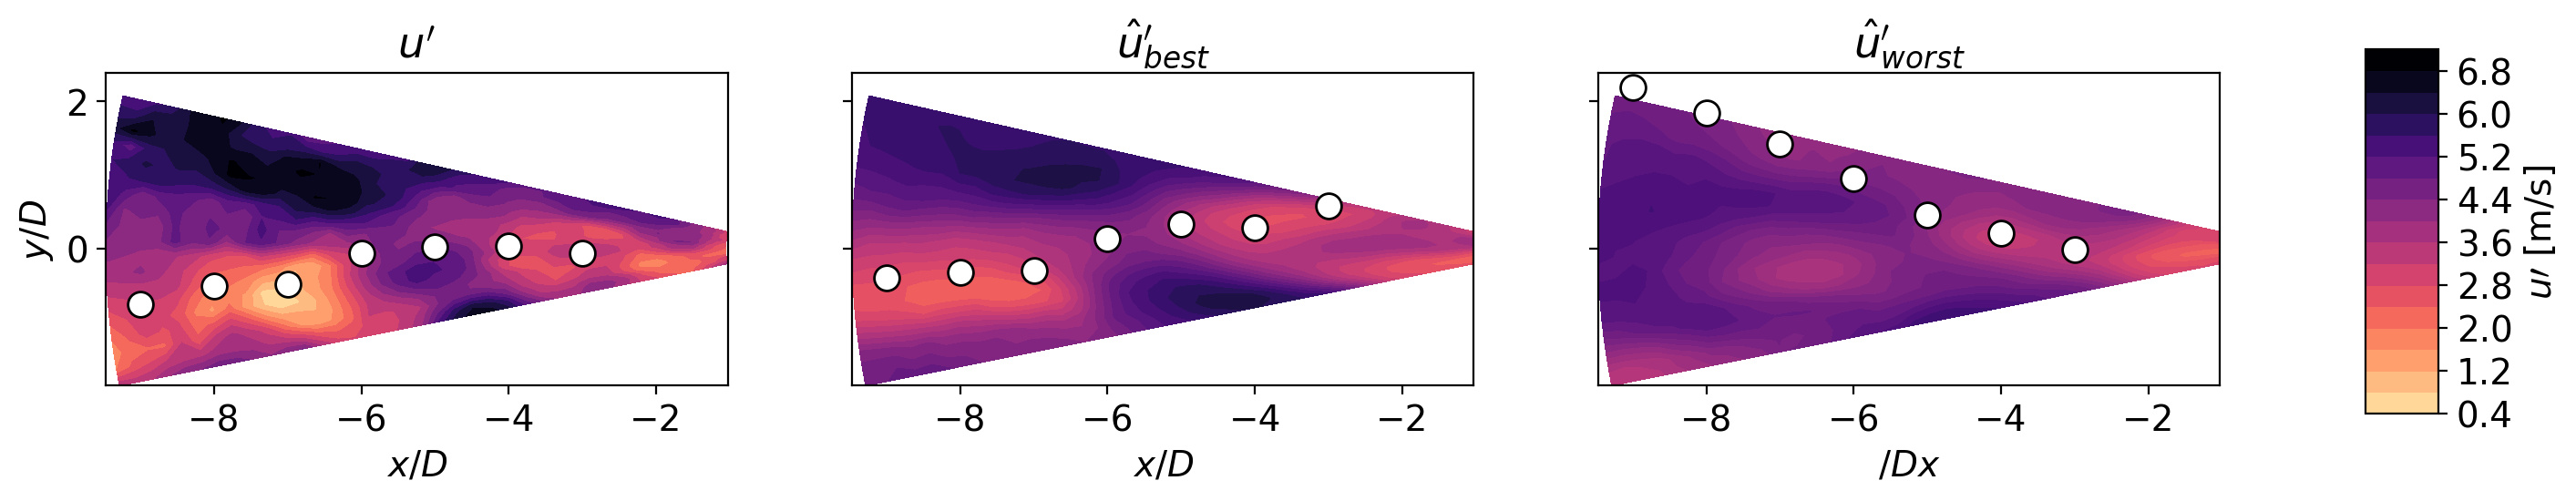
\includegraphics[width=\textwidth]{figs/C_rec_best_worst.png}
  \caption{Velocity field from Case A (left) along with the best (center) and worst (right) reconstructions with 7 modes.}
  \label{fig:fieldrec}
\end{figure}

The inflow Strouhal number, $St_\text{in}=D/U_\text{hub}\cdot T $, defined with the rotor diameter, the hub-height inflow velocity, and the inverse of the integral time scale represents the cutoff frequency for the externally-driven meandering hypothesis.
In this hypothesis, any turbulent motions in the inflow occurring at a frequency at or below $St_\text{in}$ are assumed to carry the momentum deficit of the wake as a passive tracer.
In practice, this requires that any the frequencies of the wake meandering must also be at or below the inflow Strouhal number. 
The comparison of $St_\text{in}$ to spectra of the detected wake centers  ($P_\text{wake}$) in \cref{fig:wakeSpectra} does not show an entirely clear picture of the response for $x/D \in [3,6,9]$.
While the peaks of spectra, shown as dots, for Cases B and C (orange and gray) occur below $St_\text{in}$, shown as vertical lines, this relationship does not hold for Case A.
The cause for the unexpected behavior in the wake center location spectra for Case A is not immediately clear, but may be related to the change of operating conditions seen during that time period. 

\begin{figure}[htb]
    \centering
    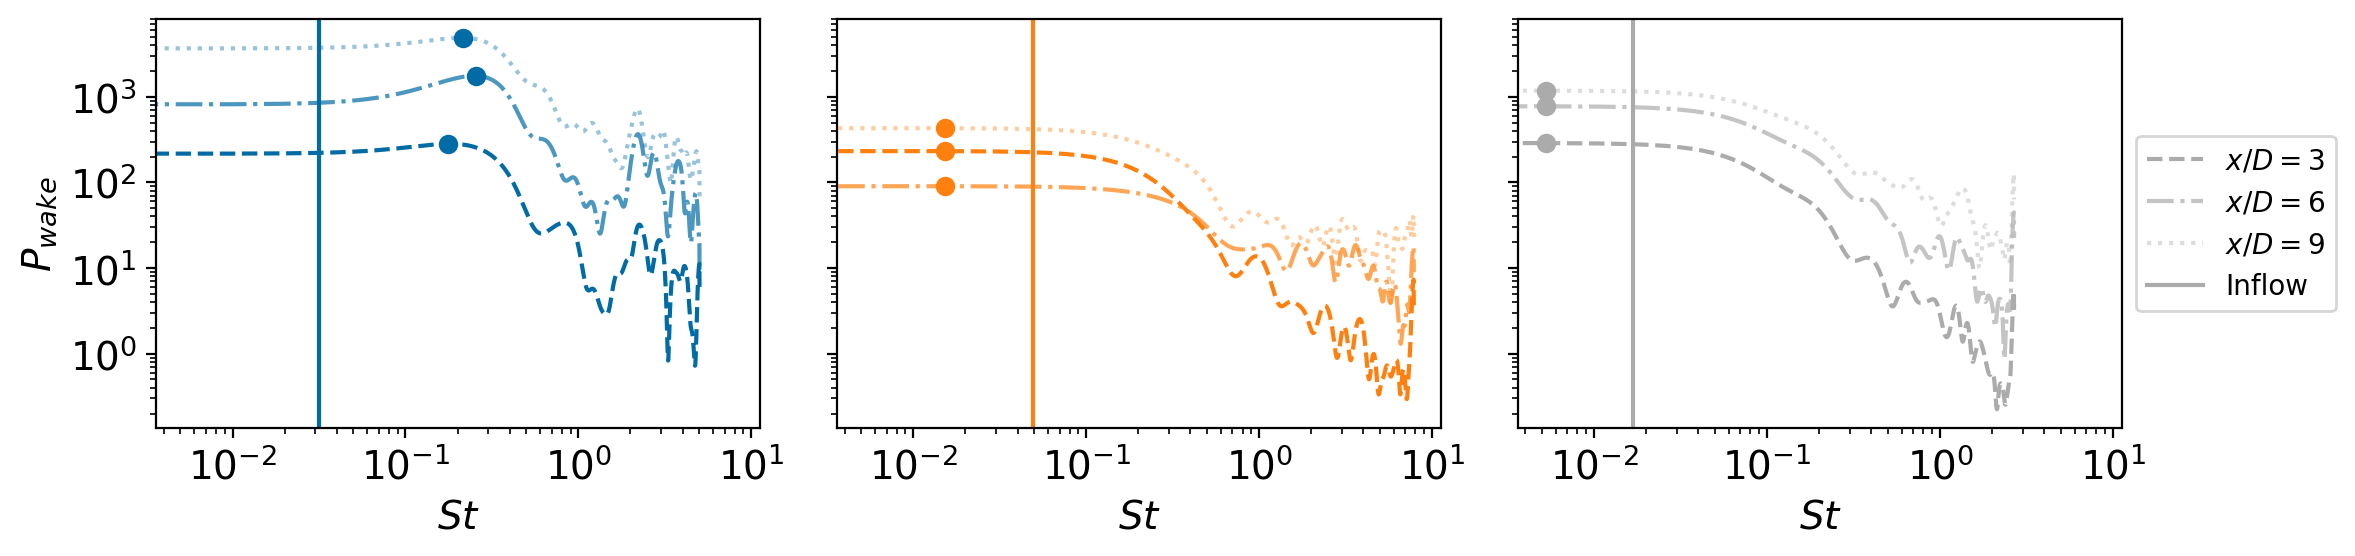
\includegraphics[width=\columnwidth]{figs/wake_spectra.png}
    \caption{Wake center spectra from the lidar scans in Strouhal scaling. The vertical line in each plot shows $St_\text{in}$ for Cases A, B, and C, from left.}
    \label{fig:wakeSpectra}
\end{figure}

POD modes themselves are functions only of space, all time dependence of each structure is contained in the mode amplitudes $a_i(t)$, as in \cref{eqn:POD}.
Computing the power spectral density (PSD) for each mode coefficient ($P_{a_i}$) highlights the spectral contribution of each mode in the reduced-order description of the wake.
For each mode, the Strouhal number associated with the maximum value of the PSD is taken as the characteristic dimensionless frequency for each mode, $St_\text{wake}$, noting that the maximum frequency resolved is half that of the the lidar scans $f_\text{max} = f_\text{scan}/2 \approx  0.07$ Hz. For each mode coefficient, frequencies are described in Strouhal scaling as $St = f\cdot D/U_\text{hub}$.

The maximum Strouhal number for each mode depends on the average hub-height velocity for each case. 
\Cref{fig:bestworstcoeff} shows the PSDs of the POD coefficients associated with the modes highlighted by the regression coefficients in \cref{fig:regression}.
For each case, the modes most closely associated with wake meandering---those with the largest negative values of $\beta$---are shown on the left. 
PSDs of coefficients that contribute least to the reconstruction of wake meandering are shown on the right.
Note that modes are listed in the order of the greatest (left) and least (right) contributions, and are different for each case.
For each mode, a point of the same color indicates the maximum value of the PSD and the characteristic Strouhal number, $St_{a_i, \text{c}}$.

\begin{figure}[h]
  \centering
  \begin{subfigure}[b]{0.49\columnwidth}
    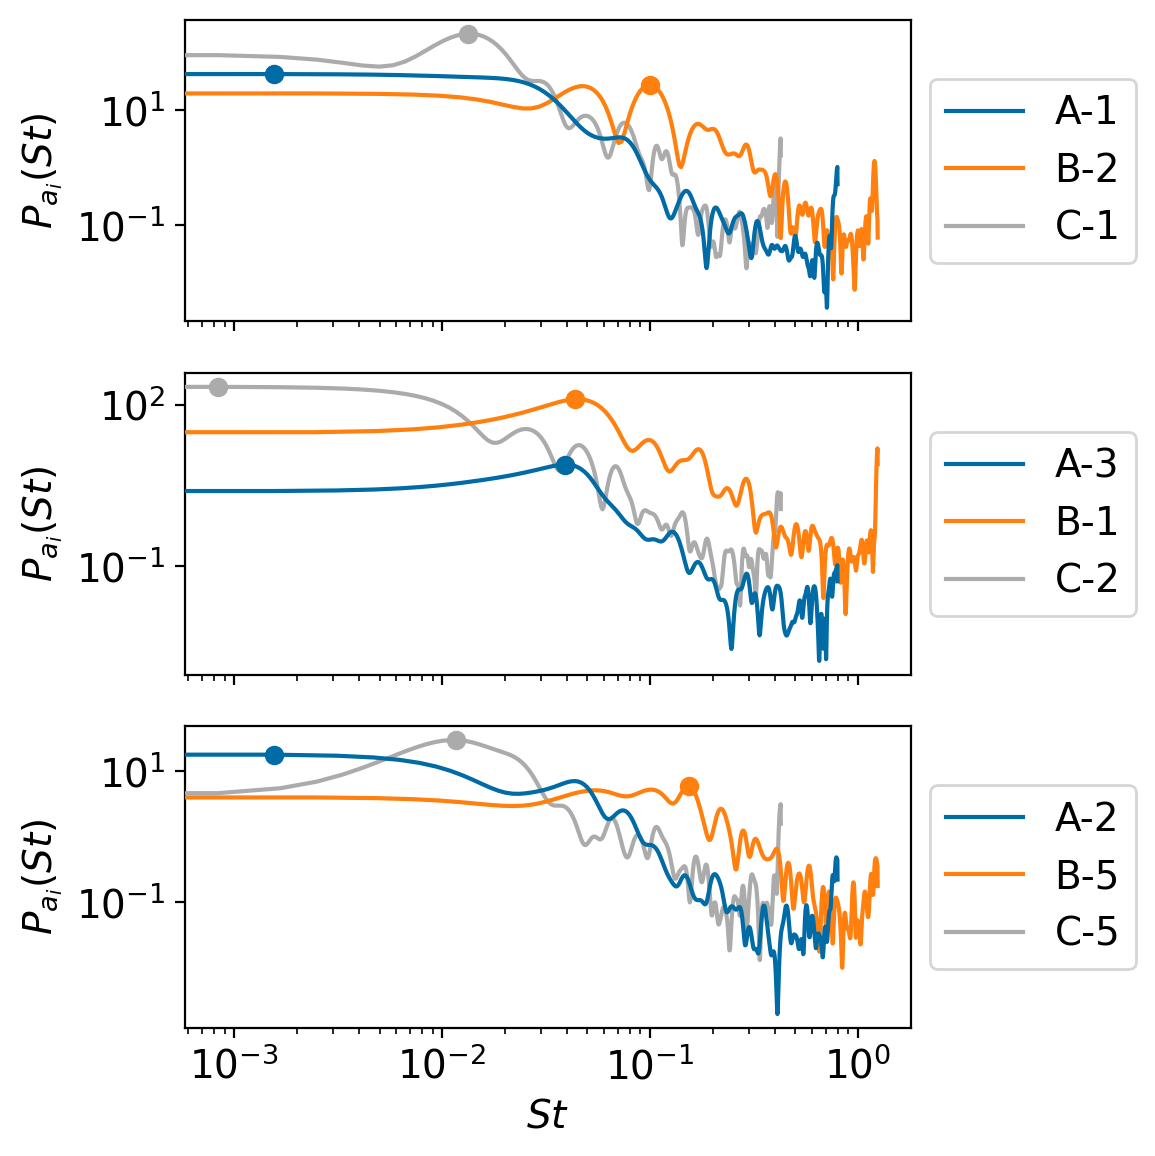
\includegraphics[width=\columnwidth]{figs/best_coeff_st.png}
  \end{subfigure}
  \begin{subfigure}[b]{0.49\columnwidth}
    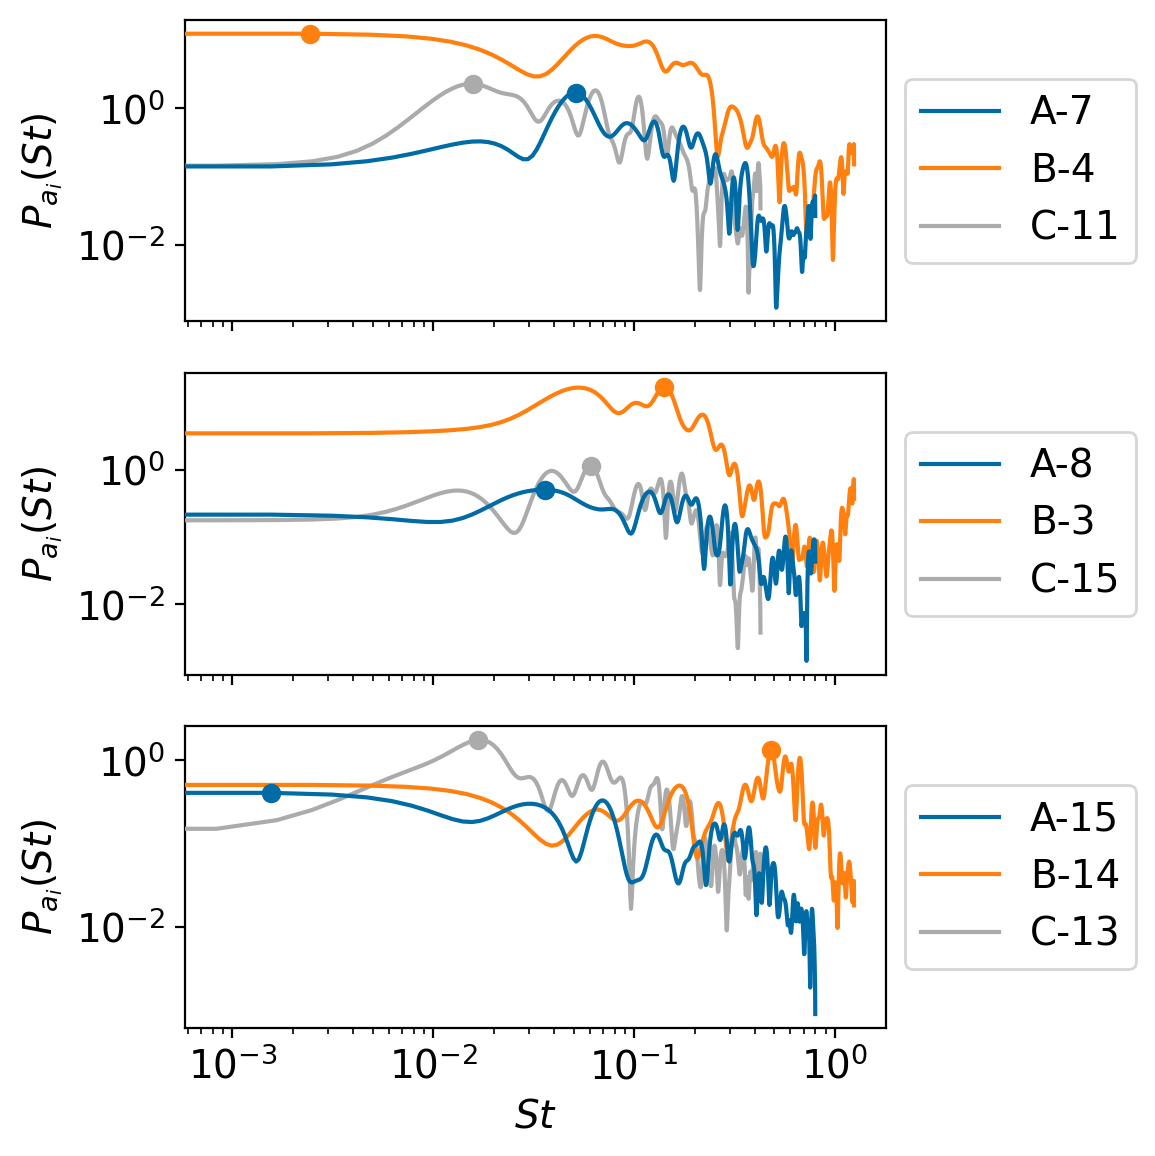
\includegraphics[width=\columnwidth]{figs/worst_coeff_st.png}
  \end{subfigure}
  \caption{PSDs of POD projection coefficients ($a_i$) for the modes that contribute most (left) and least (right) to wake meandering.}
  \label{fig:bestworstcoeff}
\end{figure}

The spectra shown in \cref{fig:bestworstcoeff} associated with an accurate representation of wake meandering (left) consistently show peaks of $St_{a_i, \text{c}} < 0.2$, agreeing with dominant meandering frequencies in previous work,
\cite{medici2008measurements,okulov2007stability, okulov2014regular,howard2015statistics,foti2016wake,foti2018wake,baker1985wake,zambrano1983wake,larsen2007dynamic,larsen2008wake,jonkman2017development}
but the relationship is less clear for modes that contribute little to meandering (right).
\Cref{fig:ST_comp} compares the $St$ associated with spectral peaks for the POD modes in all cases to those of the inflow (solid lines) and those observed in the wakes (dashed lines).
Spectral peaks shown with open diamonds are those from the POD modes that correspond most with the accurate reconstruction of the wake meandering, filled circle markers are all other modes considered for velocity field reconstruction.
\begin{figure}[htb]
    \centering
    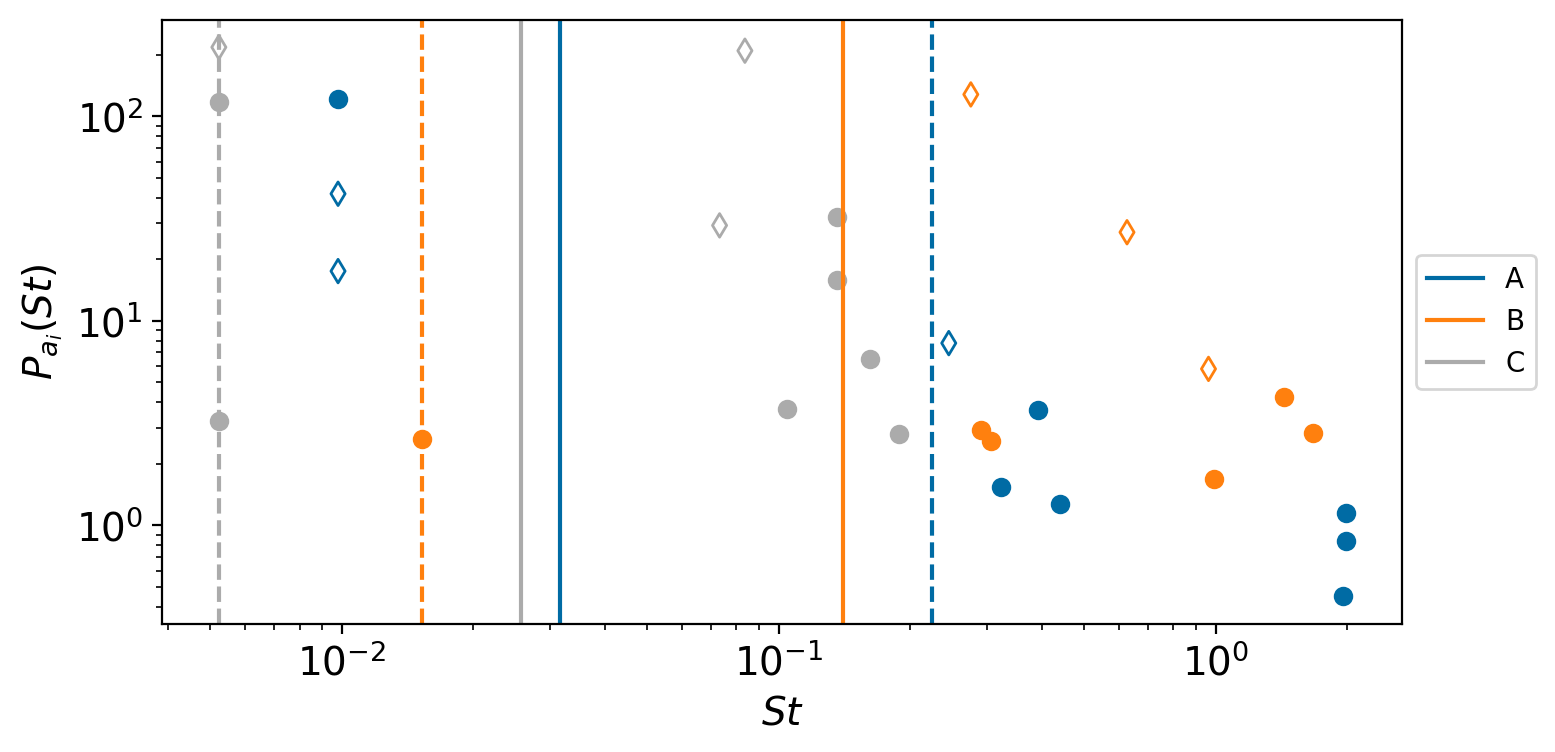
\includegraphics[width=0.8\columnwidth]{figs/ST_comparison.png}
    \caption{Peak $St$ derived from POD mode coefficients for each case. Diamond markers are the modes that contribute most to meander, circle markers are modes that contribute less. The solid vertical lines are $St_\text{in}$, dashed vertical lines are $St_\text{wake}$.}
    \label{fig:ST_comp}
\end{figure}
As with the spectra in \cref{fig:wakeSpectra}, the results comparing $St_{a_i,\text{c}}$ for individual modes in \cref{fig:ST_comp} are not entirely consistent with the externally-driven meandering hypothesis. 
For that to be the case, we would expect $St_{a_i,\text{c}}$ to be more cleanly divided by $St_\text{in}$, with modes that contribute to the accurate reconstruction of the wake (diamonds) at $St_{a_i,\text{c}} < St_\text{in}$ and modes that contribute little to meandering to have $St_{a_i,\text{c}} > St_\text{in}$.
Instead, we see a mix of $St_{a_i,\text{c}}$, where some of the modes that contribute least to meander have the lowest characteristic frequencies.

Similarly, following the internally-driven meandering hypotheses, those that assert that wake meandering is a product of interactions between turbulent structures in the wake, we would expect modes that contribute to meandering to have frequencies near those of the wake meandering detected from the lidar scans.
Because the POD identifies coherent turbulent structures, like hub and tip vortices, it is reasonable to expect that their interactions should be characterized by the POD modes and coefficients. 
However, values of $St_{a_i,\text{c}}$ do not show any consistent behavior related to $St_\text{wake}$ either.
Although tip and hub vortices are typically associated with characteristic frequencies higher than are resolved with the lidar scans, their interactions should be on the same order of magnitude as the wake meandering. 



\section{Conclusions} % (fold)
\label{sec:Conclusions}

The use of remote sensing data  from scanning lidars in wind turbine wake research gives us an opportunity to examine wake dynamics at full scale. 
Measurements are guaranteed to align with the atmospheric flow and with the wind turbine wake by mounting the lidar on the nacelle.
This work uses high-speed horizontal sector scans from a nacelle-mounted lidar to assess the wake meandering dynamics of a utility scale wind turbine operating in three different inflow conditions.
Wake center locations, detected downstream of the wind turbine by fitting a Gaussian profile to the wake, show different meandering statistics in each of the test cases.
In this work, we quantify wake meandering in a spatiotemporal sense with snapshot POD and in a spectral sense by seeking characteristic dimensionless meandering frequencies. 

The Snapshot POD describes coherent turbulent structures in the wake, along with their relative contribution to the overall TKE budget and a coefficient that describes their dynamics.
In this work, we exhaustively examine the reconstructed wake flow by selecting subsets of POD modes in a combinatorial sense, and compare meandering statistics to those shown in the lidar scans.
Our work shows that, contrary to expectation, the lowest ranking modes do not necessarily contribute most to the accurate representation of wake meandering.
Although the lowest order modes represent the largest, most coherent turbulent structures, they are not uniformly present in the combinations that best represent wake meandering. 

Low-dimensional representations of the flow field are simply linear combinations of POD modes and their respective coefficients, indicating that the final flow field depends linearly on each mode.
A regression test between modes and meandering statistics suggests that some modes are completely disconnected from meandering dynamics, and still others that actively work \emph{against} accurately representing wake meandering in low-dimensional flow reconstructions.
Moreover, some of the best-fit reconstructions may consistently fail to accurately describe the wake center at particular downstream locations depending on the modes used in the low-order description, indicating that some modes are relevant to different regions of the wake.

However, spectra defined from the mode coefficients most correlated with describing wake meandering do not exhibit the expected relationship with the characteristic Strouhal numbers of the inflow or of the wake.
Dynamics wake meandering models that treat the momentum deficit in the wake as a passive tracer assume that wake motion is driven by atmospheric turbulence above a certain cutoff frequency, and so the Strouhal numbers for significant modes should be lower than that of the inflow.
Those that say wake meandering is a product of the interaction between coherent turbulent structures in the wake should expect to see a relationship between the characteristic Stouhal numbers of the wakes and those of the modes.
Unfortunately, neither relationship is evident in the results of the current study, either because the structures that describe meandering are not adequately resolved by the measurements, or because wake meandering has a more complex relationship with turbulence in the wake and inflow than noted in the literature.




% section Conclusions (end)

\section*{Acknowledgements}

This work was authored in part by the National Renewable Energy Laboratory, operated by Alliance for Sustainable Energy, LLC, for the U.S. Department of Energy (DOE) under Contract No. DE-AC36-08GO28308. Funding provided by the U.S. Department of Energy Office of Energy Efficiency and Renewable Energy Wind Energy Technologies Office. The views expressed herein do not necessarily represent the views of the DOE or the U.S. Government. The U.S. Government retains and the publisher, by accepting the article for publication, acknowledges that the U.S. Government retains a nonexclusive, paid-up, irrevocable, worldwide license to publish or reproduce the published form of this work, or allow others to do so, for U.S. Government purposes. 


\bibliography{refs}
% \nocite{*}

\end{document}
%
% ****** End of file aipsamp.tex ******
